\documentclass{interact}

%\usepackage{epstopdf}% To incorporate .eps illustrations using PDFLaTeX, etc.
\usepackage[caption=false]{subfig}% Support for small, `sub' figures and tables
%\usepackage[nolists,tablesfirst]{endfloat}% To `separate' figures and tables from text if required

%\usepackage[doublespacing]{setspace}% To produce a `double spaced' document if required
%\setlength\parindent{24pt}% To increase paragraph indentation when line spacing is doubled
%\setlength\bibindent{2em}% To increase hanging indent in bibliography when line spacing is doubled

\usepackage[numbers,sort&compress]{natbib}% Citation support using natbib.sty
\bibpunct[, ]{[}{]}{,}{n}{,}{,}% Citation support using natbib.sty
\renewcommand\bibfont{\fontsize{10}{12}\selectfont}% Bibliography support using natbib.sty

%\theoremstyle{plain}% Theorem-like structures provided by amsthm.sty
%\newtheorem{theorem}{Theorem}[section]
%\newtheorem{lemma}[theorem]{Lemma}
%\newtheorem{corollary}[theorem]{Corollary}
%\newtheorem{proposition}[theorem]{Proposition}

%\theoremstyle{definition}
%\newtheorem{definition}[theorem]{Definition}
%\newtheorem{example}[theorem]{Example}

%\theoremstyle{remark}
%\newtheorem{remark}{Remark}
%\newtheorem{notation}{Notation}

\begin{document}

\articletype{REVIEW ARTICLE}% Specify the article type or omit as appropriate

\title{The integrated nested Laplace approximation applied to spatial log-Gaussian Cox process models}

\author{
\name{Kenneth Flagg\thanks{CONTACT Kenneth Flagg. Email: kenneth.flagg@montana.edu} and Andrew Hoegh}
\affil{Montana State University, Bozeman, MT}
}

\maketitle

\begin{abstract}
Spatial point process models are theoretically useful for mapping discrete
events, such as plant or animal presence, across space; however, the computational
complexity of fitting these models is often a barrier to their practical use.
The log-Gaussian Cox process (LGCP) is a point process driven by a latent
Gaussian field, and recent advances have made it possible to fit Bayesian LGCP
models using approximate methods that facilitate rapid computation. These advances
include the integrated nested Laplace approximation (INLA) with a
stochastic partial differential equations (SPDE) approach to
sparsely approximate the Gaussian field and an extension using pseudodata with
a Poisson response. To help link the theoretical results to statistical
practice, we provide an overview of INLA for point process data 
and then illustrate their implementation using freely available data. 
The analyzed datasets include both a completely observed spatial field
 and an incomplete data situation. Our well-commented R
code is shared in the online supplement. Our intent is to make these methods
accessible to the practitioner of spatial statistics without requiring deep
knowledge of point process theory.
\end{abstract}

\begin{keywords}
Bayesian hierarchical model, INLA, spatial prediction, log-Gaussian Cox process, spatial point process
\end{keywords}


\section{Introduction}
\label{intro}

Statistical methods for spatial prediction result in a high-dimensional
inference problem that can present computational challenges, particularly for
large datasets. For instance, when the goal of statistical modeling is to
produce a graphical map of a random variable over space, the model ultimately
must be able to predict that random variable at every pixel of the image. A map
image will typically be at least several hundred by several hundred pixels, so
in total there can easily be hundreds of thousands of pixels requiring
predictions. Thus, even when a model has only half a dozen parameters, spatial
prediction may require hundreds of thousands of latent variables.

Spatial point process models further complicate the situation; in addition to
computational challenges due to a large number of latent variables and
parameters, point process models also require evaluating difficult
likelihoods. Both maximum likelihood and Bayesian model fitting require
integrating the intensity function over space, but the integral is generally
not available in closed form and, unlike a probability distribution, the
integral over the entire domain does not necessarily equal one.

Many methods have been introduced for modeling spatial point patterns,
including Poisson regression approximations, maximum pseudolikelihood, and
Markov chain Monte
Carlo~\cite{bermanturner,baddeleyetal,baddeleyturner,moellerwaagepetersen}.
The number of parameters and latent variables in these models still poses a
major computational challenge. This computational challenge led to the
development of the integrated nested Laplace approximation (INLA).

INLA was introduced by Rue, Martino, and Chopin (2009), who sought fast and
accurate posterior approximation for Bayesian additive regression models with
Gaussian latent fields and allowing for non-Gaussian responses~\cite{rueetal}.
This setting includes random effects models, generalized linear models, spline
models, dynamic models, spatial and spatiotemporal models, among others.
A non-Gaussian response in one of these models typically results in the
posterior having no closed form. The standard solution for analyzing these
data is MCMC. However, INLA is much faster; Rue,
Martino, and Chopin showed that INLA can find accurate and precise
approximations in minutes or seconds when MCMC would take days or hours to
achieve similar precision.

Development of INLA has made accurate approximate model fitting considerably
more feasible for a particular class of log-Gaussian Cox process (LGCP)
models. {\bf Early work applying INLA to LGCP models included studying replicated point patterns for syphilis risk \cite{li2012log} and muskoxen locations \cite{illian2012using}.} A key part of INLA's computational simplicity is that it calculates
the posterior distribution of each latent Gaussian variable one at a time;
that is, it provides only the posterior marginal distributions rather than the
full joint distribution.

When using a LGCP model for spatial mapping, two aspects make INLA a suitable
approach. First, the LGCP is driven by a spatial Gaussian process (GP), so the
latent variables are Gaussian. Second, even though the latent variables are
expected to exhibit spatial dependence, their full joint distribution is not
needed. In most situations it suffices to map their predicted values, variance,
and upper and lower interval bounds pointwise across space.

We focus on spatial mapping using a hierarchical construction of the LGCP, and
do so without discussing many classic spatial point process concepts such as
Gibbs processes, Markov processes, point process densities, or the Papangelou
conditional intensity function. For readers interested in the general spatial
point process context in which the LGCP originates, we recommend other
references~\cite{moellerwaagepetersen, digglepoint, cressie}.

Recently, there has been renewed interest in fitting LGCP models to
incompletely-observed point patterns, known in the point process literature as
variable sampling effort. This scenario arises when analysts seek to map the
intensity across some domain, but cannot census every event in the domain.
Instead, effort is made to observe events in certain sections of the domain.
Either a subregion of the domain is sampled or a random subset of the events
are sampled. The subregion situation commonly occurs when quadrat sampling is
employed or when the domain is partitioned into areal regions and only certain
regions can be surveyed. The random subset situation is best known from
distance sampling, where a set of line transects are traversed and all events
detected near the transects are recorded. The events are assumed to be detected
with a probability depending on the distance from the transect. Hybrids of the
subregion and random subset situation are possible when there is a hard limit
to the distance at which events can be observed, for example because some
equipment cannot leave the transect. Point patterns observed under variable
sampling effort have traditionally been aggregated to the quadrat, transect,
or grid cell level before analysis~\cite{digglepoint}. However, INLA aids the
fitting of LGCP models to such data.

This article provides a review of recent advances in the fitting of spatial
LGCP models via INLA, including a finite element approach for dimension
reduction, a likelihood factorization that avoids gridding, and incorporation
of sampling effort or false negatives. The examples use freely-available
datasets and the R code is provided in the supplementary materials. The remainder of
Section~\ref{intro} provides an overview of spatial LGCP
models and INLA. Section~\ref{methods} describes the methodology developed to
fit LGCP models in INLA, and Section~\ref{application} presents example
analyses of real-world data. Finally, Section~\ref{conclusion} presents
concluding remarks.

\subsection{Log-Gaussian Cox Process}
\label{lgcp}

The log-Gaussian Cox process is a Poisson process driven by a latent Gaussian
process~\cite{moelleretal}. This section provides a brief overview of the
spatial Poisson process and then presents the hierarchical construction of the
spatial LGCP.

A spatial point process generates a random set of events (points) in space.
The process is characterized primarily by its intensity function
\(\lambda(u)\), which gives the local mean number of events per unit area at
any point in space. The intensity function is nonnegative and defined on a
domain \(\mathcal{D} \subset \mathbb{R}^{2}\). The point process is observed
in a bounded window \(\mathcal{R} \subset \mathcal{D}\). The point process is
denoted \(\mathbf{X}\), and its realizations are \(\mathbf{x} = \{x_{1},
\dots, x_{n}\}\). A realized (observed) \(\mathbf{x}\) is called a point
pattern; the elements of the point pattern are the events.

The Poisson process is fully defined by its intensity function and satisfies
the following two properties \cite{moellerwaagepetersen}:
\begin{enumerate}
\item The number of events in any region \(\mathcal{B}\) follows a Poisson
distribution with mean
\(\int_{\mathcal{B}} \lambda(u)\mathrm{d}u\).
\item Given the number of events in \(\mathcal{B}\), those events are
independent and identically distributed with probability density
\(\lambda(u) / \int_{\mathcal{B}} \lambda(u)\mathrm{d}u\).
\end{enumerate}
The distribution function of a Poisson process is
\begin{equation}
\pi(\mathbf{X}|\lambda)
= \frac{\exp\left[-\int_{\mathcal{R}} \lambda(u) \mathrm{d}u\right]}{n!}
\prod_{x \in \mathbf{X}} \lambda(x)
\end{equation}
as given in Cressie (1993) \cite{cressie}. This can be extended to include
further parameters used to define \(\lambda\), most commonly coefficients
to construct a log-linear model with covariates, or a polynomial or spline
function of the spatial coordinates. In a Poisson process, the intensity 
function is a fixed parameter (or a
deterministic function of fixed parameters and covariates). In applications of
spatial point process models, this is often too simplistic because spatial
heterogeneity may be driven by other random processes with their own parameters
about which inferences are desired.

A Cox process is a generalization of the Poisson process where the intensity
function is a realization of another stochastic process~\cite{cox,digglepoint}.
Conditional on the intensity function, a Cox process must satisfy the two
Poisson process properties, but the intensity function can take any form. Cox
processes are commonly used to model clustering of events, such as in the
classic Neyman-Scott process where cluster centers are generated by another
Poisson process~\cite{neymanscott}. Another example is where the intensity is
a Dirichlet process mixture~\cite{taddy,flagg2020}. In situations where the intensity
function is less structured but exhibits spatial autocorrelation, the Cox
process can incorporate a geostatistical process; the log-Gaussian Cox process
is an example of this.

The LGCP uses a log-linear model for the intensity
\begin{equation}
\log\lambda(u) = \boldsymbol{\Psi}(u)
= \mathbf{z}(u)' \boldsymbol{\beta} + \mathbf{e}(u),
\end{equation}
where \(\mathbf{e}\) is a Gaussian process with mean 0 and covariance function
\(C(u, v)\). Where the spatial Poisson process has a (stochastically) 
fixed intensity to be
estimated from data, the spatial LGCP induces a hierarchical model where the
intensity function is itself a random process to be predicted.

Spatial or spatiotemporal LGCP models have recently been applied to whale
populations (Yuan et. al., 2017), landslides (Lombardo et. al., 2018), fMRI
data (Samartsidis et. al., 2019), {\bf unemployment estimates (Pereira 2019 et. al., 2019), wildfile mapping (Serra et. al., 2014)} and disease mapping (Konstantinoudis et.
al., 2020) to list only a few
applications~\cite{yuanetal,lombardoetal,samartsidisetal,pereira2019,serra2014,konstantinoudisetal}.
Baddeley et. al.~(2005) and M\"{o}ller and Waagepetersen~(2007) present model
checking tools for LGCP and other spatial point process
models~\cite{baddeleyresiduals,moellerwaagepetersen}.


\subsection{Integrated Nested Laplace Approximation}
\label{inla}

INLA was developed with the goal of providing fast, accurate, deterministic
approximations for posterior marginal distributions of the parameters in
latent Gaussian models~\cite{rueetal}. The setting is Bayesian generalized
additive models but is kept very general; this includes linear models, models
with nonlinear (spline, random walk, etc.) functions of predictors, and models
with temporal and/or spatial dependence. Such models commonly include many
Gaussian latent variables or parameters with Gaussian priors and relatively
few non-Gaussian parameters. The INLA approach makes repeated use of Laplace
expansion, numerical integration, and numerical search. The method has
established usefulness for the LGCP~\cite{illianetal}. It is readily implemented
using the standalone INLA software or in R via the R-INLA
package~\cite{inlar}.

Our objective in this section is to provide an overview of the mathematical
motivation behind INLA while omitting technical details that can be found
elsewhere. The notation used in this section is somewhat nonstandard, but
consistent with spatial point process notation. Let \(\mathbf{y}\) be the
response (vector). Let \(\boldsymbol{\xi}\) be a vector of all unobserved
Gaussian variables in the model, including both parameters with Gaussian
priors, and latent Gaussian variables such as random effects or values of a
Gaussian field to be predicted. { \bf (Note S$\o$rbye et. al. (2019) provides guidance on prior specification \cite{s2019})}. Let \(\boldsymbol{\theta}\) be a vector of all
non-Gaussian model parameters. The posterior distribution is
\begin{equation}
\pi\left(\boldsymbol{\xi}, \boldsymbol{\theta}| \mathbf{y}\right)
= \frac{\pi\left(\mathbf{y}, \boldsymbol{\xi}, \boldsymbol{\theta}\right)}
{\int \pi\left(\mathbf{y}, \boldsymbol{\xi}, \boldsymbol{\theta}\right)
\mathrm{d}\mathbf{y}}
\end{equation}
but the integral is not available in closed form, so the posterior must be
either sampled from or approximated. The INLA approach is to first find a
Laplace approximation of \(\pi\left(\boldsymbol{\theta} | \mathbf{y}\right)\).
Then, that result and a further Laplace expansion are used to approximate each
posterior marginal \(\pi\left(\xi_{i}| \mathbf{y}\right)\), where \(\xi_{i}\)
is the \(i\)th latent Gaussian variable in \(\boldsymbol{\xi}\).

The derivation begins by invoking the definition of conditional probability,
rewriting
\begin{equation}
\pi\left(\boldsymbol{\theta} | \mathbf{y}\right)
\propto \frac{\pi\left(\mathbf{y}, \boldsymbol{\xi}, \boldsymbol{\theta}\right)}
{\pi\left(\boldsymbol{\xi} | \mathbf{y}, \boldsymbol{\theta}\right)}.
\end{equation}
The Laplace approximation is applied the to denominator, taking a second-order
Taylor expansion of
\(\log\left[\pi\left(\boldsymbol{\xi} | \mathbf{y}, \boldsymbol{\theta}\right)\right]\)
around the posterior mode of \(\boldsymbol{\xi}\) and then exponentiating. The
result is a Gaussian approximation of
\(\pi\left(\boldsymbol{\xi} | \mathbf{y}, \boldsymbol{\theta}\right)\). Then
the approximate posterior marginal distribution of \(\boldsymbol{\theta}\) is
\begin{equation}
\tilde{\pi}\left(\boldsymbol{\theta} | \mathbf{y}\right)
\propto \left.\frac{\pi\left(\mathbf{y}, \boldsymbol{\xi}, \boldsymbol{\theta}\right)}
{\pi_{G}\left(\boldsymbol{\xi} | \mathbf{y}, \boldsymbol{\theta}\right)}
\right|_{\boldsymbol{\xi}=\boldsymbol{\xi}^{*}}
\end{equation}
with \(\boldsymbol{\xi}^{*}\) denoting the posterior mode of
\(\boldsymbol{\xi}\).

A similar process is repeated for the posterior marginal of each \(\xi_{i}\),
beginning with
\begin{equation}
\pi\left(\xi_{i} | \mathbf{y}, \boldsymbol{\theta}\right)
\propto \frac{\pi\left(\mathbf{y}, \boldsymbol{\xi}, \boldsymbol{\theta}\right)}
{\pi\left(\boldsymbol{\xi}_{-i} | \xi_{i}, \mathbf{y}, \boldsymbol{\theta}\right)}
\end{equation}
where the \(-i\) notation indicates that the \(i\)th element is omitted from
the vector. The Laplace approximation of this denominator is still complicated,
but further approximations make it tractable. The takeaway is that, by
handling the Gaussian latent variables one at a time, computation can be made
considerably simpler compared to methods that approximate the joint posterior.

These approximations, as well as fast numerical integration methods and
numerical optimization to find the posterior modes, are packaged in the INLA
software and R-INLA library. The software offerings are stable and documented
to the point that the applied statistician can use them without knowing all of
the computational details. { \bf Rue et. al. (2017) provides a helpful review of INLA \cite{rue2017bayesian}.}


\section{Methodology}
\label{methods}

INLA provides an efficient computational framework for fitting Bayesian models
with latent Gaussian variables. On top of this framework, several tools are
built to further simplify fitting spatial LGCP models. The stochastic
partial differential equation (SPDE) approach provides dimension reduction for
the spatial GP~\cite{lindgrenetal}. The SPDE approach employs a numerical
integration scheme which can also be used to approximate the LGCP likelihood
and negate the need to grid the events into Poisson counts~\cite{simpsonetal}.
With these computational improvements, researchers are now able to efficiently
fit LGCP models to large spatial point pattern datasets and even
incompletely-observed point patterns~\cite{yuanetal}. {\bf Recently Jullum (2020) has further explored this integral approximation and made recommendations for an analytical approach than can be more accurate \cite{jullum2020}.}


\subsection{The SPDE Approach}
\label{spde}

Because the LGCP includes a Gaussian process (GP), efficient computation for
Gaussian processes is critical when working with LGCP models. The GP imposes a
dense covariance matrix on the latent variables~\cite{rinla}. For GPs with a
Mat\'{e}rn covariance function, a Gaussian Markov random field (GMRF)
approximation can simplify computation, requiring only a sparse covariance
structure. {\bf Simpson, Lindgren, and Rue (2012) frame this idea through the lens of using a continuously specified Markovian Gaussian random fields induced by a SPDE \cite{simpson2012think}. More explicitly, Simpson, Lindgren, and Rue (2012) also showed that the Gaussian Markov random field was a better representation than kernel convolution \cite{simpson2012order}.}

The GMRF approximation is motivated by the fact that Gaussian fields with
Mat\'{e}rn covariances are solutions to the stochastic partial differential
equation (SPDE) below~\cite{lindgrenetal}:
\begin{equation}
\tau(\kappa^{2} - \Delta)^{\alpha / 2} \mathbf{e}(u) = \mathbf{W}(u),
\qquad u \in \mathbb{R}^d, \quad \kappa > 0,
\quad \alpha = \nu + d/2, \quad \nu > 0
\end{equation}
Here, \(\mathbf{W}\) is a Gaussian white noise process with variance 1, and
\(\Delta\) is the Laplacian operator. The stationary solution
\(\mathbf{e}\) is a Gaussian field having a Mat\'{e}rn covariance
function with precision (inverse variance) \(\tau\),  scaling parameter
\(\kappa\) (inversely proportional to the effective range), and smoothness
parameter \(\nu\).

Lindgren, Rue, and Lindstr\"{o}m~(2011) investigate the limit as \(\nu \to 0\) for
\(d = 2\), finding that the solution is a GMRF on a unit
lattice~\cite{lindgrenetal}. They then construct approximations for positive
integer values of \(\nu\) by \(\nu\)-fold convolution of \(\mathbf{e}\)
with itself. Finally, they use a finite element method to generalize the
approximation to arbitrary triangulations of the support. This approximation
has considerable computational benefits because the GMRF has a sparse
covariance structure; the only nodes with nonzero covariances are those
directly connected by edges in the triangulation.

The core of the SPDE approach is the finite-element GMRF representation of the
GP. The idea is to model the GP at the nodes (vertices) of a triangular mesh.
Values at points other than the nodes are found by linear interpolation,
resulting in a surface constructed from triangular faces.

\begin{figure}[t!]
\centering
\subfloat[Example Gaussian process realization.]
{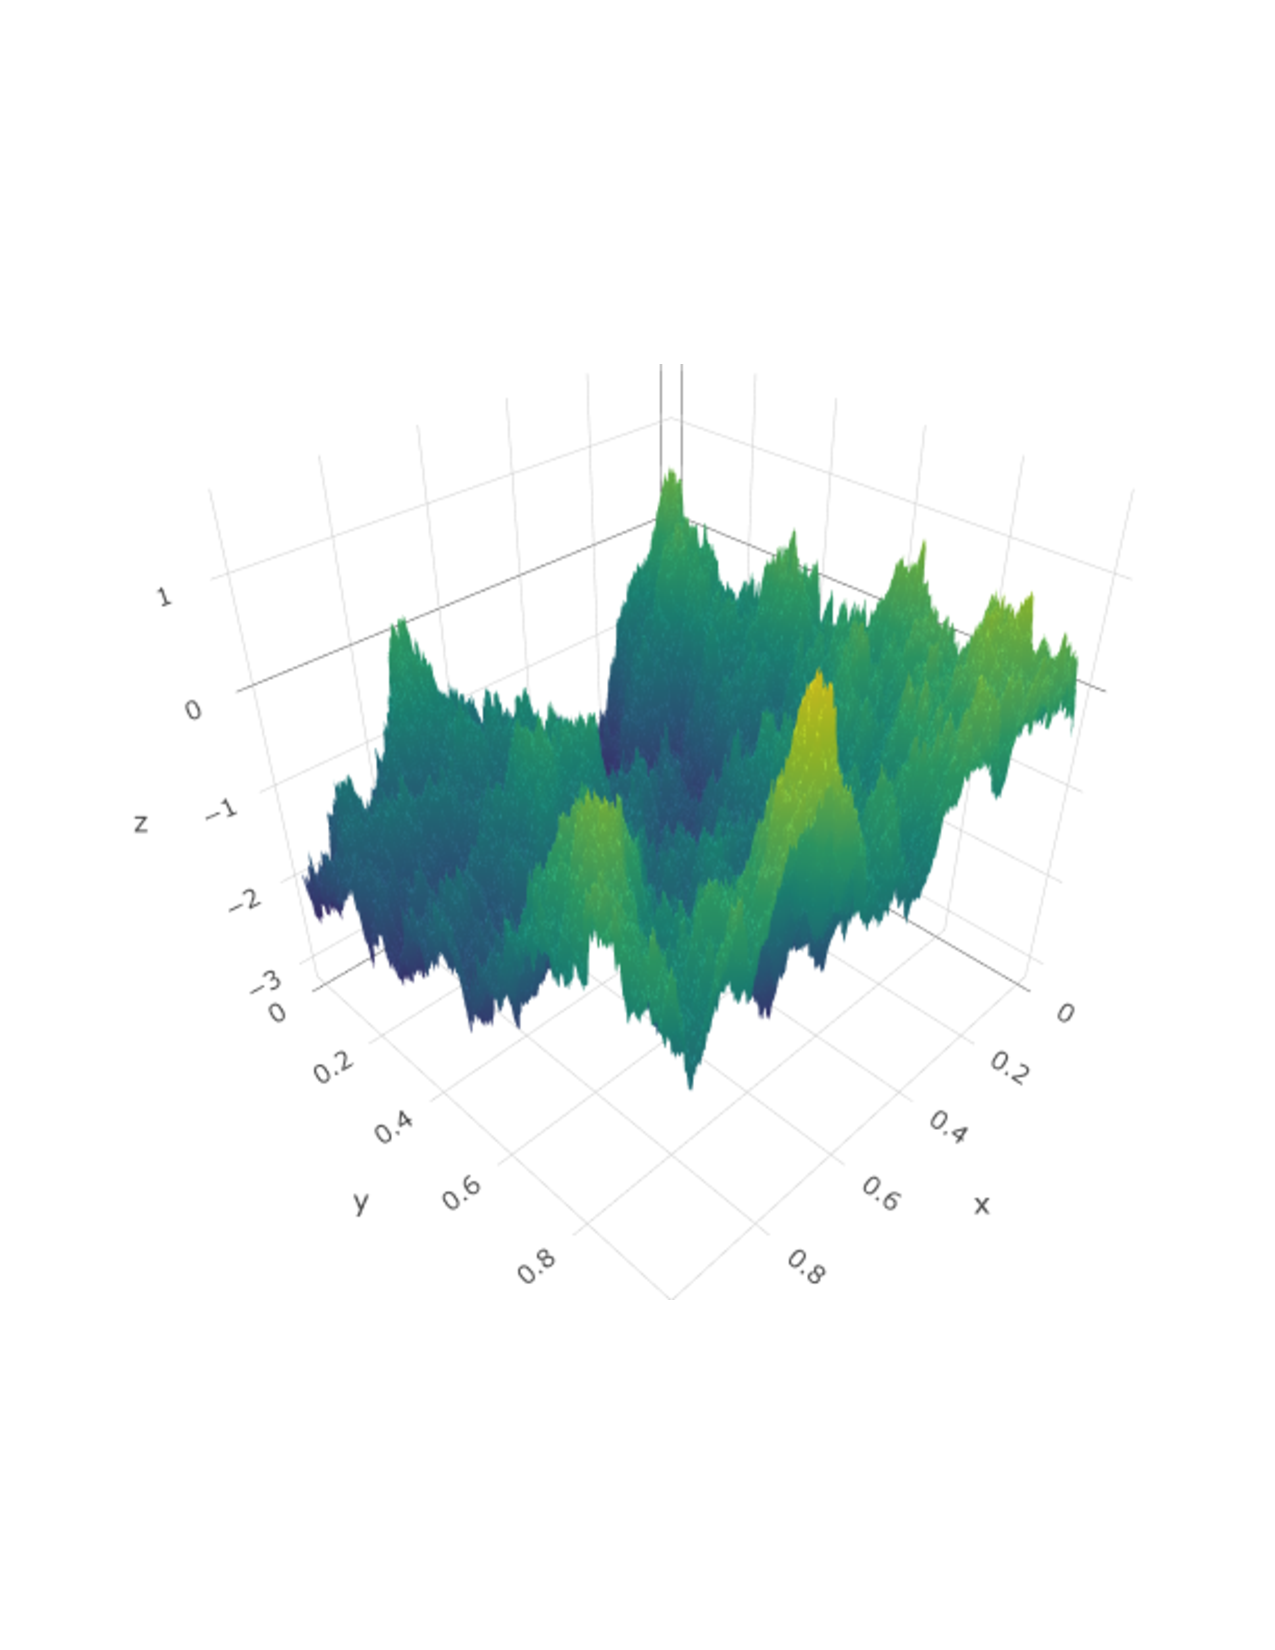
\includegraphics[width=0.4\textwidth]{figures/surface.pdf}}
\subfloat[Finite element approximation.]
{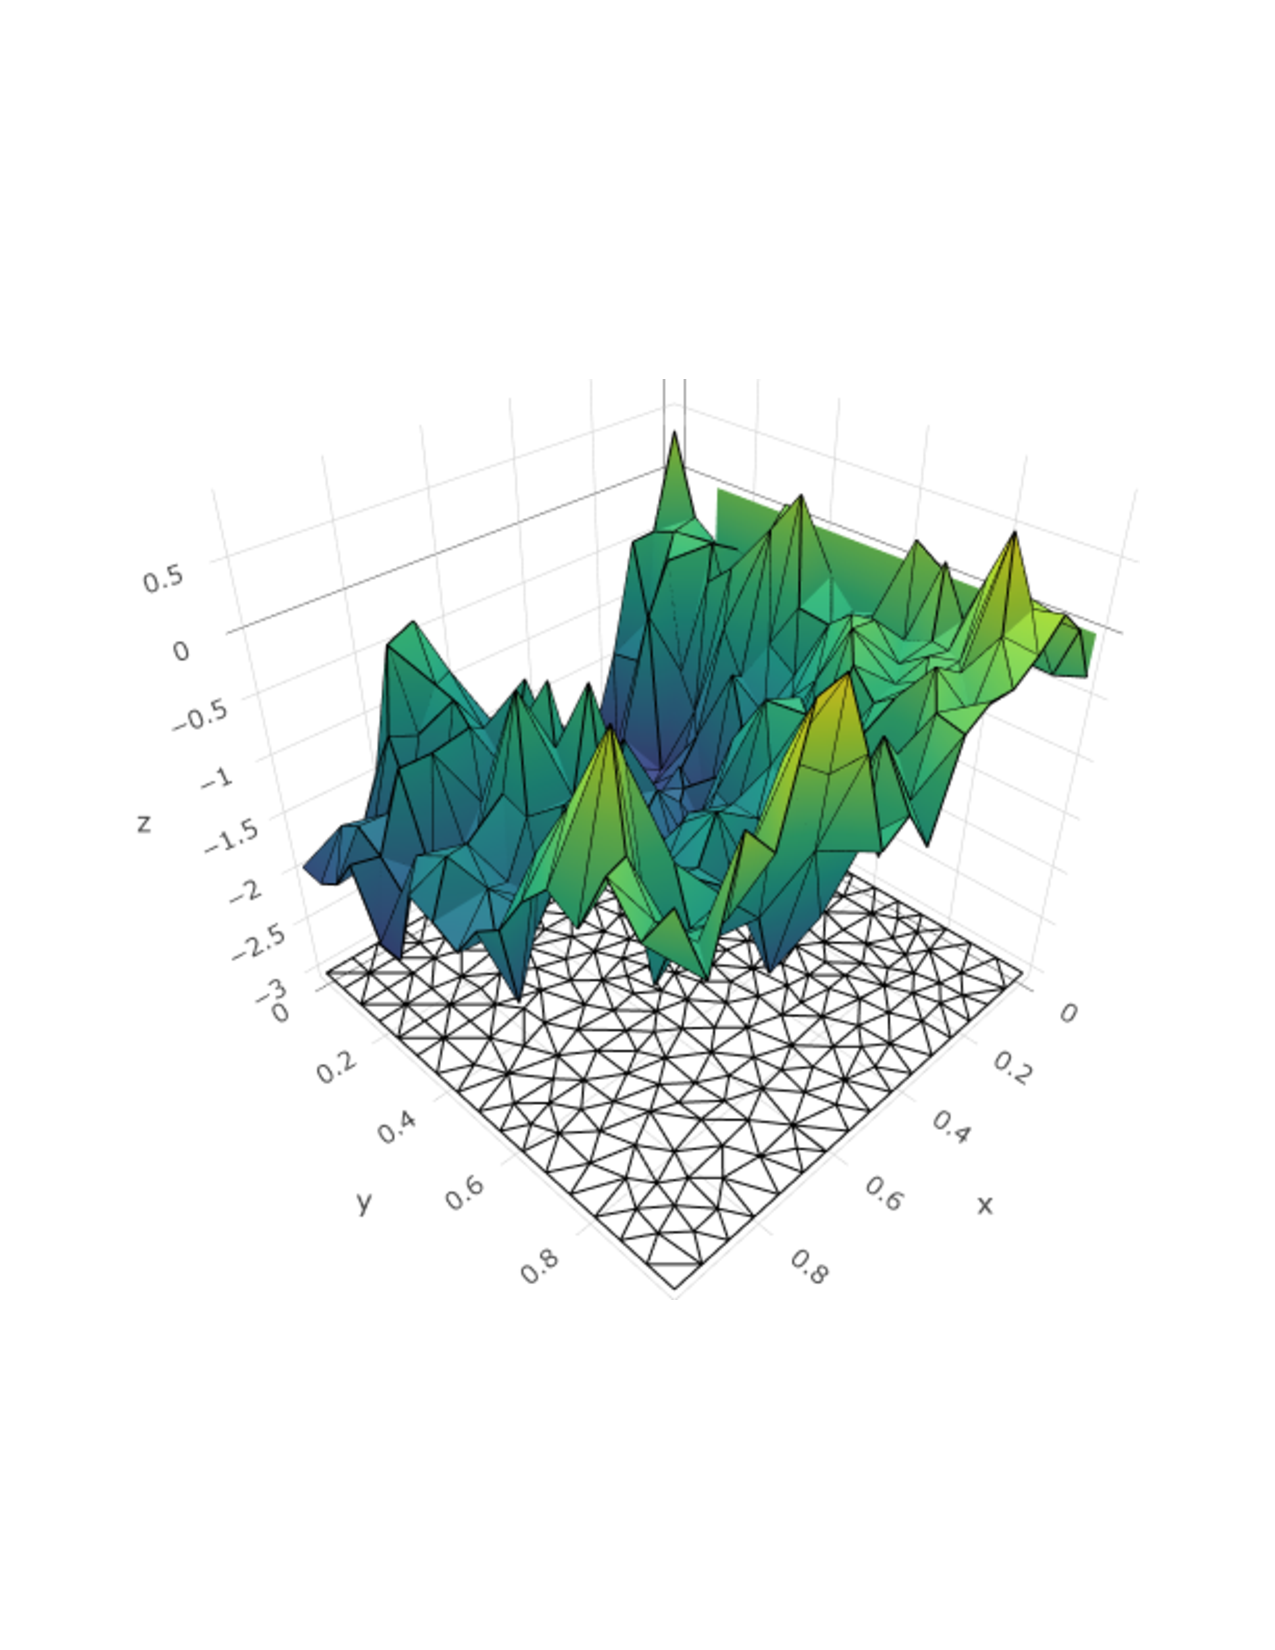
\includegraphics[width=0.4\textwidth]{figures/interp.pdf}}

\caption{A realization of a spatial Gaussian process and an
approximation of that realization over a triangular mesh.}
\label{surface}
\end{figure}
Figure~\ref{surface}
shows an example. The linear interpolation uses the barycentric coordinate
system~(Figure~\ref{triangle}). The mathematical form of this interpolation is
very simple; for a point \(u\) with barycentric coordinates \((\alpha, \beta,
\gamma)\) inside a triangle with vertices \(s_{1}, s_{2}, s_{3}\), the
approximation is simply
\begin{equation}
\mathbf{e}(u) \approx \alpha \mathbf{e}(s_{1})
+ \beta \mathbf{e}(s_{2}) + \gamma \mathbf{e}(s_{3}).
\end{equation}
This technique can approximate complicated surfaces as relatively
low-dimensional vectors via a piecewise-linear approximation.


\begin{figure}[t!]\centering

\subfloat[A point \(u\) in a triangle with vertices \(s_{1}, s_{2}, s_{3}\).]
{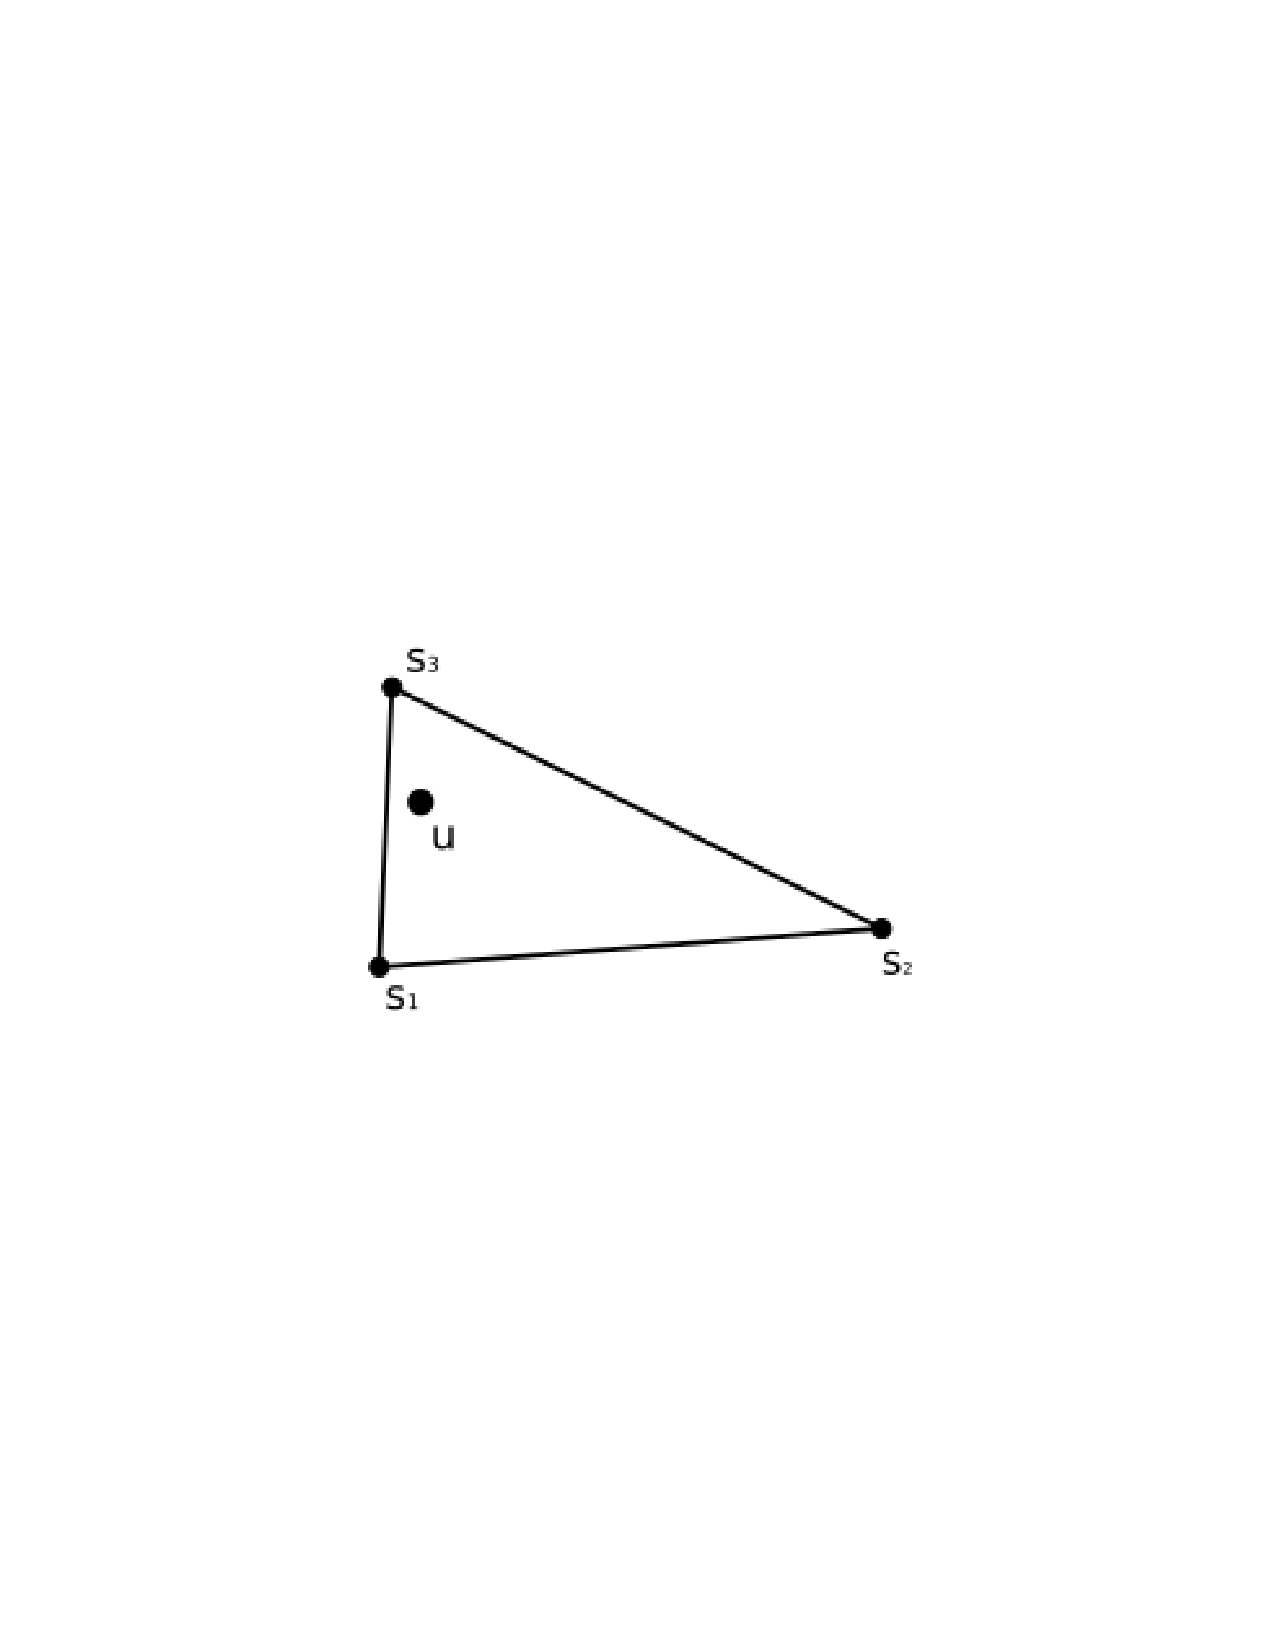
\includegraphics[width=0.3\textwidth]{figures/triangle.pdf}}
\hspace{2em}
\subfloat[A point \((\alpha, \beta, \gamma)\) in a simplex with vertices
\((1, 0, 0), (0, 1, 0), (0, 0, 1)\). ]
{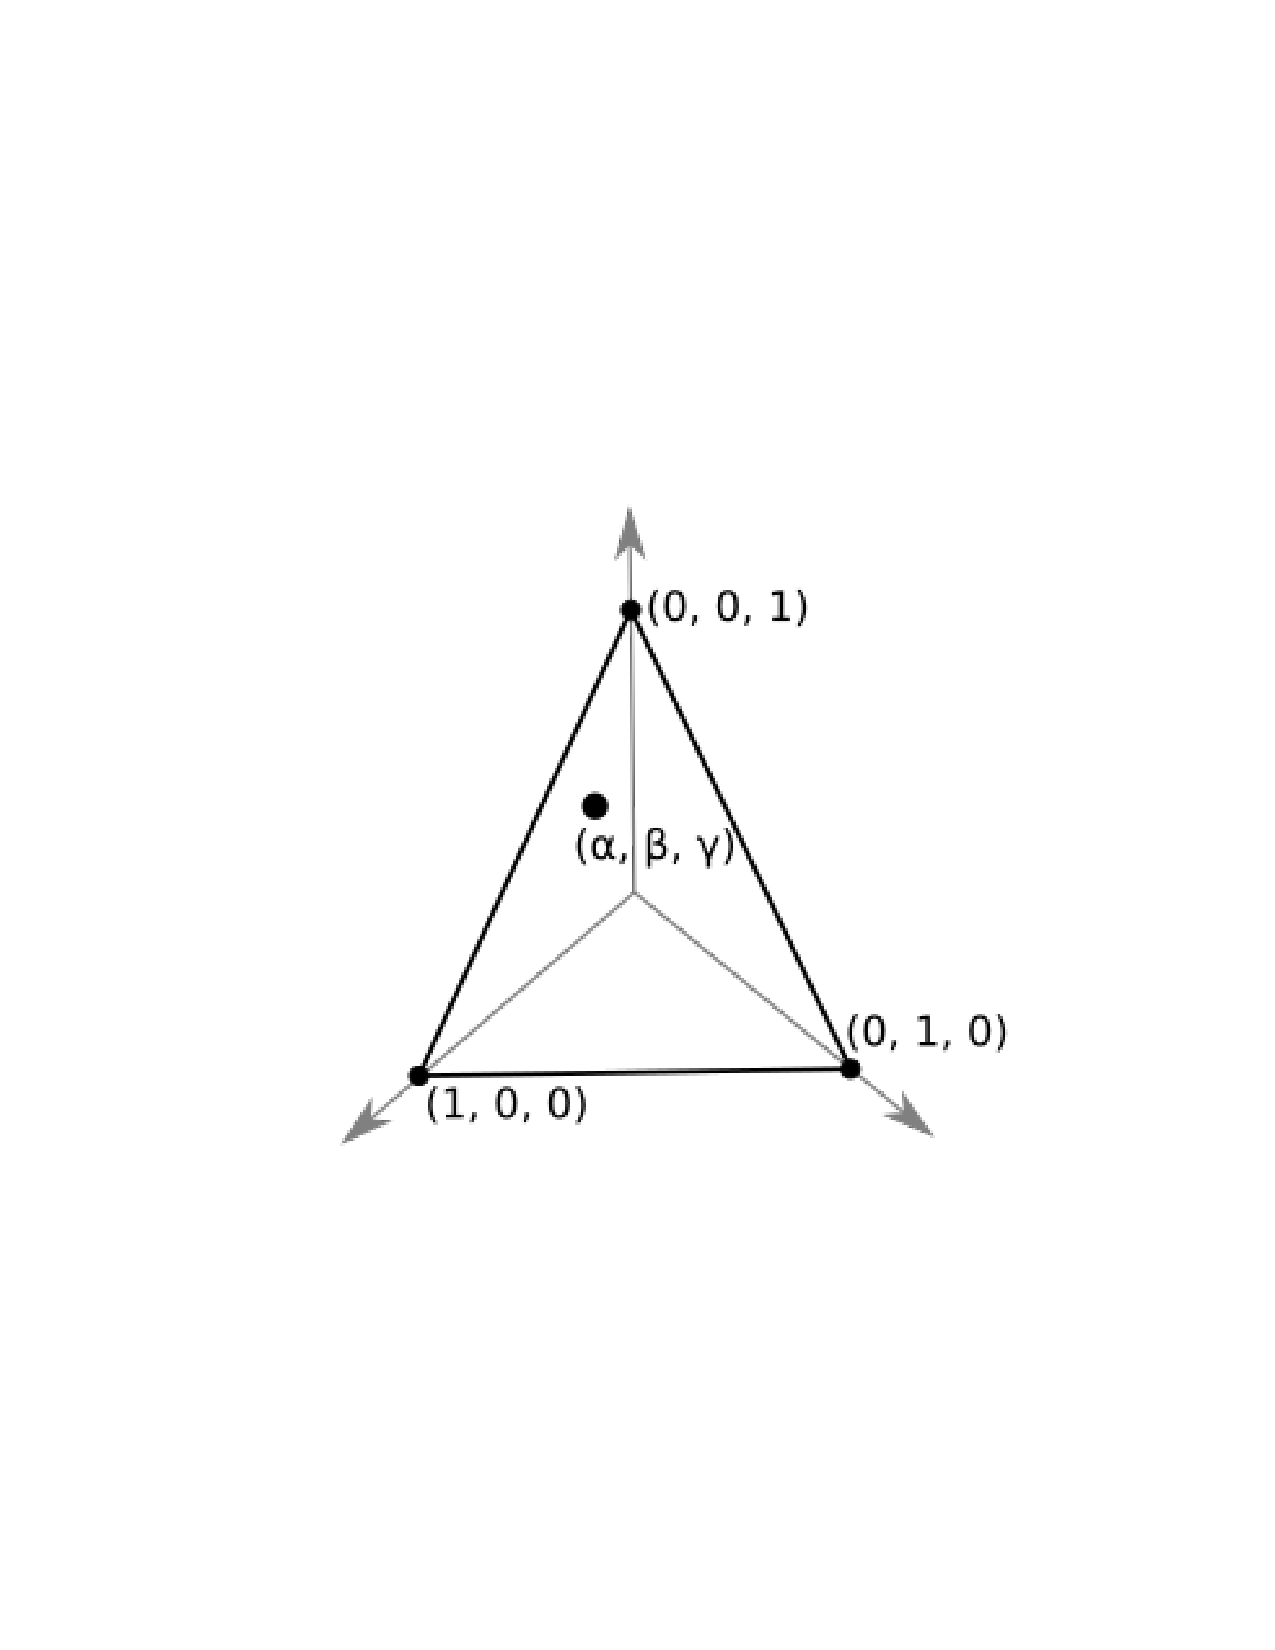
\includegraphics[width=0.3\textwidth]{figures/simplex.pdf}}

\caption{An illustration of the linear transformation from a mesh triangle to
the 2-simplex. The transformation is defined from \(\mathbb{R}^{2}\) to
\(\mathbb{R}^{3}\) such that the vertices are mapped to a unit vector along
each axis. This transformation takes the point \(u\) to
\((\alpha, \beta, \gamma)\), its barycentric coordinates. The barycentric
coordinates have the property that \(\alpha + \beta + \gamma = 1\).}
\label{triangle}
\end{figure}

\begin{figure}[t!]\centering
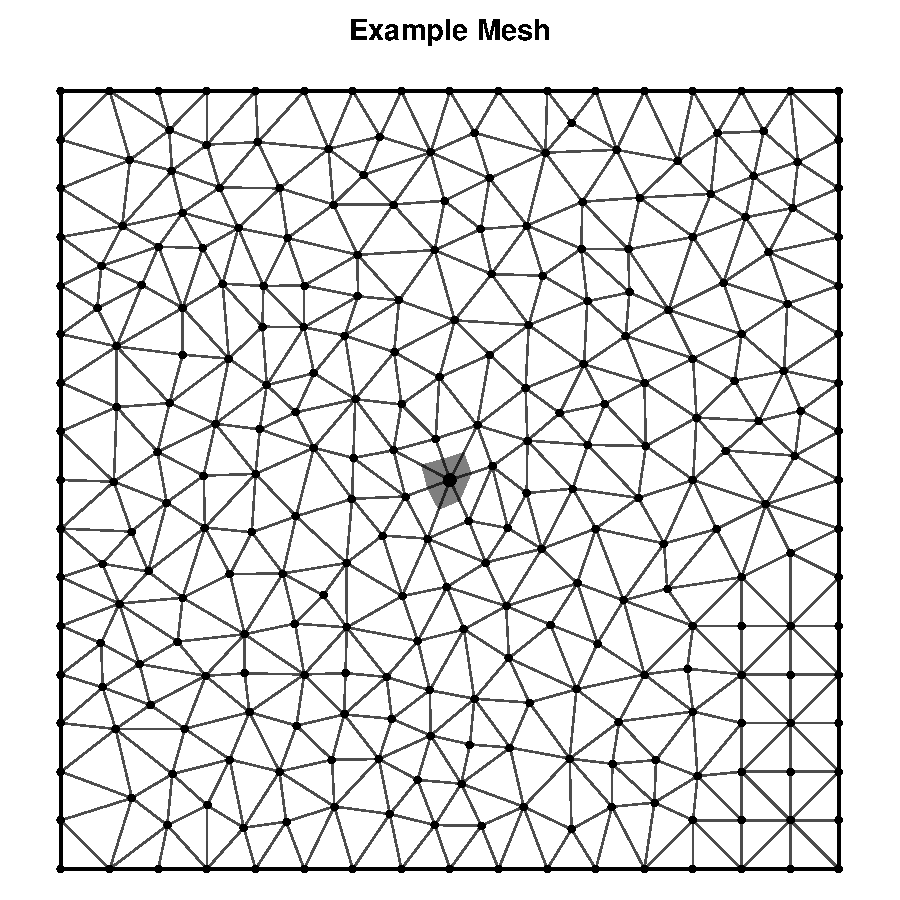
\includegraphics[width=0.3\textwidth]{figures/dual.pdf}
\caption{An illustration of the nodes (dots) and the weighting scheme for one
node (large dot). In the SPDE approach, this node represents it dual region
(shaded), so its weight is proportional to the shaded area. The dual region is
constructed by connecting the midpoints of the node's edges to the centroids
of the adjacent triangles.}
\label{dual}
\end{figure}

The full finite element representation is constructed in the following manner.
Start with a triangular mesh over the spatial domain, with nodes
\(s_{1}, \dots, s_{m}\). Then define a set of basis functions
\(\{\phi_{1}, \dots, \phi_{m}\}\) that map the spatial domain to the
barycentric coordinate system. That is, \(\phi_{i}\) corresponds to node
\(s_{i}\), and for a point \(u\) there are at most three nonzero
\(\phi_{i}(u)\). The nonzero values give the barycentric coordinates of \(u\)
in a triangle containing it. The finite element representation has the form
\begin{equation}
\mathbf{e}(u) \approx \sum_{j = 1}^{m} \psi_{j} \phi_{j}(u).
\end{equation}
The vector \(\boldsymbol{\psi} = (\psi_{1}, \dots, \psi_{m})'\) is a
realization of the GMRF, so it is a multivariate Gaussian vector comprised of
the values of the latent field at the nodes.

The \(\psi_{i}\) values are used to compute averages and for numerical
integration, in which cases they are weighted by the area represented by the
nodes~(Figure~\ref{dual}). The region represented by a node is called its dual
region, denoted \(\mathrm{dual}(s)\) for node \(s\). The dual region is
constructed by connecting the midpoints of the edges and centroids of the
triangles for which the node is a vertex. The weight is the area of the dual
region, which is one third of the total area of the triangles used in its
construction.

In practice, the SPDE approach goes as follows. Choose nodes \(s_{i}\)
at which to model \(\boldsymbol{\Psi}(s_{i})
= \mathbf{z}(s_{i})' \boldsymbol{\beta} + \mathbf{e}(s_{i})\), then build a
triangular mesh using these nodes. Typically the nodes will include locations
where data or covariates are available, then the rest will be filled in with a
Delaunay triangulation under some edge length constraints. The
\(\mathbf{e}(s_{i})\) are modeled as a GMRF where the distribution of
each \(\mathbf{e}(s_{i})\) depends only on the
\(\mathbf{e}(s_{j})\) where \(s_{i}\) and \(s_{j}\) are connected by an
edge. The GMRF representation is assumed to be a piecewise linear approximation
of the continuous Gaussian field;

The SPDE approach is implemented in the R-INLA package alongside tools
for constructing meshes. A wrapper for easily specifying LGCP models is
provided in the \texttt{inlabru} package~\cite{inlabru}. { \bf A recent textbook contains additional information and reproducible code for using SPDE's and R-INLA \cite{krainski2018}. Furthermore, Bakka et. al. (2018) provides an review of spatial modeling for SPDEs \cite{bakka2018spatial}.}


\subsection{Going Off the Grid}
\label{offgrid}

Point pattern data are sometimes known as presence-only data, underscoring
the fact that information about where events did \emph{not} occur is both
important and often overlooked. There have been many proposed methods to
account for regions that were observed to contain no events (in contrast to
unobserved regions where it is unknown if any events are present). Many of
these methods involve imputation of dummy points or discretization. With maximum likelihood, perhaps the most well-developed of these use
approximations based on Poisson regression on presence/absence information in
small disjoint regions~\cite{bermanturner,baddeleyturner}. Another alternative, 
which is probably the most popular approach to Bayesian
fitting of LGCP models but is also common in frequentist analyses, is to grid
the domain and model the induced Poisson counts. It has long been understood
that results are sensitive to the discretization scheme~\cite{brixmoeller}.
Simpson et. al. (2016) explain that this is also computationally
wasteful~\cite{simpsonetal}.

Simpson et. al. took LGCP inference ``off grid'' by introducing a
computationally-efficient approximation to the Poisson process likelihood that
requires the intensity function only to be evaluated at the locations of
observed events and at the nodes of a mesh. Thus, the SPDE approach can be
employed to model the intensity surface and the same nodes reused in
evaluation of the Poisson process likelihood. The result is a substantial
improvement in both computing time and accuracy of the approximation compared
to gridding.

The approximation arises from a factorization of the Poisson process
likelihood. For notational clarity, assume \(\log[\lambda(u)]
= \boldsymbol{\Psi}(u)\). The exact log-likelihood is
\begin{equation}
\ell(\lambda) = C - \int \lambda(u) \mathrm{d}u
+ \sum_{i = 1}^{n} \log\left[\lambda(x_{i})\right]
\end{equation}
where \(C\) is a normalizing constant. The log-intensity is rewritten using the
GMRF representation from the SPDE approach,
\begin{equation}
\log\left[\lambda(u)\right]
\approx \sum_{j = 1}^{m} \psi_{j} \phi_{j}(u).
\end{equation}
This defines a numerical integration scheme at nodes \(s_{i}\)
with weights \(\alpha_{i}\), where the weight is the observed area in
\(\mathrm{dual}(s_{i})\), and yields the approximation,
\begin{align}
\ell(\lambda) &\approx C - \sum_{i = 1}^{m} \alpha_{i}
\exp\left[\sum_{j = 1}^{m} \psi_{j}\phi_{j}(s_{i})\right]
+ \sum_{i = 1}^{n} \sum_{j = 1}^{m} \psi_{j}\phi_{j}(x_{i}) \\
& = C - \boldsymbol{\alpha}'
\exp\left[\mathbf{A} \boldsymbol{\psi}\right]
+ \mathbf{y}' \mathbf{A} \boldsymbol{\psi}. \label{logpois}
\end{align}
We have introduced some simplifying notation. The weight vector
\begin{equation}
\boldsymbol{\alpha} = (\alpha_{1}, \dots, \alpha_{m}, 0, \dots, 0)'
\end{equation}
contains the weight for each node and then \(n\) zeros corresponding to the
events. \(\mathbf{y}\) is a pseudodata response vector with entries
\(y_{i} = 0\) corresponding to the nodes \(s_{i}\) and \(y_{m+i} = 1\) to the
events \(x_{i}\). \(\mathbf{A}\) is an \(m + n\) by \(m\) matrix where the
first \(m\) rows are the barycentric coordinates of each node and the final
\(n\) rows are the barycentric coordinates of each event.

The rewritten log-likelihood~\eqref{logpois} is equivalent to the log-likelihood of
independent Poisson random variables with means \(\alpha_{i} \eta_{i}\) and
response vector \(\mathbf{y}\). The \(\alpha_{i}\) weights play the role of
an offset. \(\eta_{i}\) is the intensity at the location of \(y_{i}\), which
is being modeled by the GMRF. Thus, the SPDE approach, which can be easily
implemented in R-INLA, can be combined hierarchically with a Poisson GLMM to
rapidly fit a LGCP model. There is no need to compute grid counts, only to
define dummy points at the mesh nodes and construct a pseudodata vector
\(\mathbf{y}\).


\subsection{Variable Sampling Effort}
\label{veffort}

There has long been a gap between point process modeling theory and practice,
where point process models are only fit to data from completely-observed
domains under the assumption that every event was detected perfectly. {\bf While R-INLA contains functionality to fit models that account for physical barriers \cite{bakka2019}, incompletely-observed domain is a different problem.} In
practice, this is not the case as it may be impossible or impractical to census
the entire region of interest. For example, line-transect surveys routinely
generate point pattern data but are analyzed after aggregation rather than
using a point process model. Another issue is that of false negatives, in other
words events which exist but are not detected during the survey. False
negatives are an accepted part of species abundance and occupancy surveys,
where the species of interest may be camouflaged or hidden in thick
cover~\cite{linkbarker,bucklandetal,mackenzieetal}.

The idea of the incompletely-observed domain has been around for some time.
Brix and M\"{o}ller (2001) fit an LGCP model to weed data observed in
rectangular frames and used a Metropolis-adjusted Langevin algorithm
to predict the intensity outside of the observed frames~\cite{brixmoeller}.
Chakraborty et. al (2011) discuss nonhomogeneous Poisson process modeling as
a richer alternative to ecological presence/absence models and describe their
data as ``degraded'' in the sense that sampling bias prevented the entire
region from being fully observed; they fit their model by aggregating the
point pattern to counts in grid cells and using MCMC~\cite{chakrabortyetal}.
Gabriel et. al. (2016, 2017) derived a relationship between the Kriging
predictor and the LGCP to predict the LGCP intensity across an unobserved
subset of the region of interest~\cite{gabrieletal2016, gabrieletal2017}. 
Flagg et. al. (2020) used a Cox model with a Dirichlet process mixture
intensity to map hot spots in unexploded ordnance data collected along
line transects~\cite{flagg2020}.

With INLA, the SPDE approach, and the ``off grid'' approximation
facilitating the routine fitting of LGCP models, there is now renewed interest
in accounting for variable sampling effort in spatial point process
models~\cite{simpsonetal,yuanetal}. Sampling effort is accounted for using the theory of thinned point processes.
Thinning refers to the events of one point process being kept or discarded
probabilistically. Let \(\lambda(u)\) be the intensity of the parent process,
and let an event \(x=u\) (if it exists) be observed with probability
\(p(u)\). The observed point process is a thinned point process with
intensity
\begin{equation}
\lambda_{p}(u) = p(u) \lambda(u) \label{thinintensity}
\end{equation}
and if the parent process is a Poisson process then the observed process is
also a Poisson process~\cite{moellerbook}.

We seek to make posterior inferences about the parent intensity,
\(\lambda(u)\). If \(p(u)\) is known, its value at each node is used to
adjust the SPDE integration weights. Most usefully, if it is known that
\(p(s) = 0\) at certain nodes \(s\) because they were outside the surveyed
domain, the weights become zero so those nodes do not contribute to the
integral. More generally, when a known subdomain is surveyed, \(p(u)\) is
an indicator function for \(u\) being in the surveyed region. When \(p(u)\)
is known, the integration weight for node \(s_{i}\) is multiplied by
\(\int_{\mathrm{dual}(s_{i})} p(u) \mathrm{d}u\)
which, for indicator functions, is simply the proportion of the dual region
that is inside the surveyed region.

If \(p(u)\) is unknown, it can be modeled. Taking the logarithm of the thinned
intensity~\eqref{thinintensity} and substituting in the basis function
representation, we have the log-linear model
\begin{equation}
\log\left[\lambda_{p}(u)\right]
= \log\left[p(u)\right] + \sum_{j = 1}^{m} \psi_{j} \phi_{j}(u).
\end{equation}
Thus, any log-linear model for \(p(u)\) that can be fit by INLA and the SPDE
approach can be incorporated into the LGCP model. This provides a convenient
way to estimate the detection function from distance sampling data; the model
for \(\log[p(u)]\) includes the distance to the nearest transect as a
covariate. For example, Yuan et. al (2017) fit such a model to data from a
line-transect survey using a spline model to account for the unknown detection
function~\cite{yuanetal}.


\section{Applications}
\label{application}

For an example analysis of real-world data, we consider the locations of
\(n = 3605\) \emph{Beilschmiedia pendula Lauraceae} trees in a 1000~meter by
500~meter plot in a tropical rainforest on Barro Colorado Island,
Panama~\cite{moellerwaagepetersen}. This dataset has appeared as an example
in several articles, including the original INLA paper where the events were
aggregated to grid cell counts. We present an analysis that does not use
aggregation.

The data are available as the \texttt{bei} dataset in the \texttt{spatstat} R
package~\cite{spatstat}. The point pattern is accompanied by elevation and
gradient covariates measured on a square lattice with 5 m spacing. The point
pattern exhibits inhomogeneity which appears to be associated with elevation
and the elevation gradient~(Figure~\ref{bei}).


\begin{figure}[p!]\centering

\subfloat[Locations of trees (events).]
{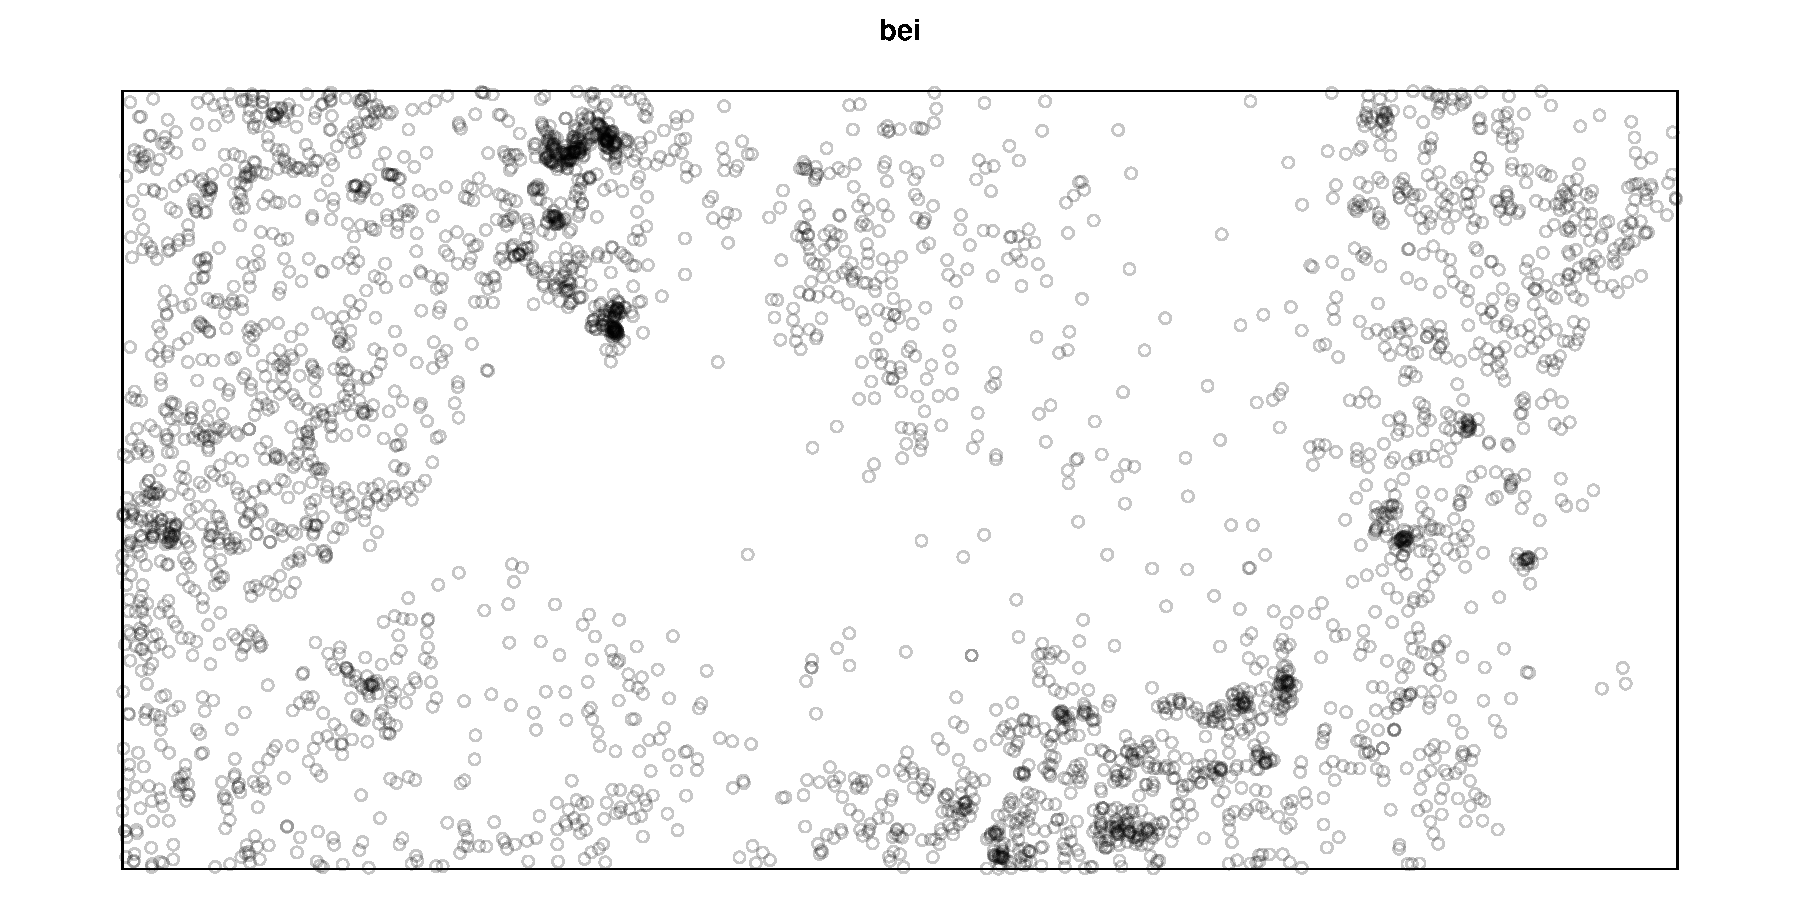
\includegraphics[width=0.9\textwidth]{figures/bei.pdf}}

\subfloat[Elevation in meters, with events overlaid.]
{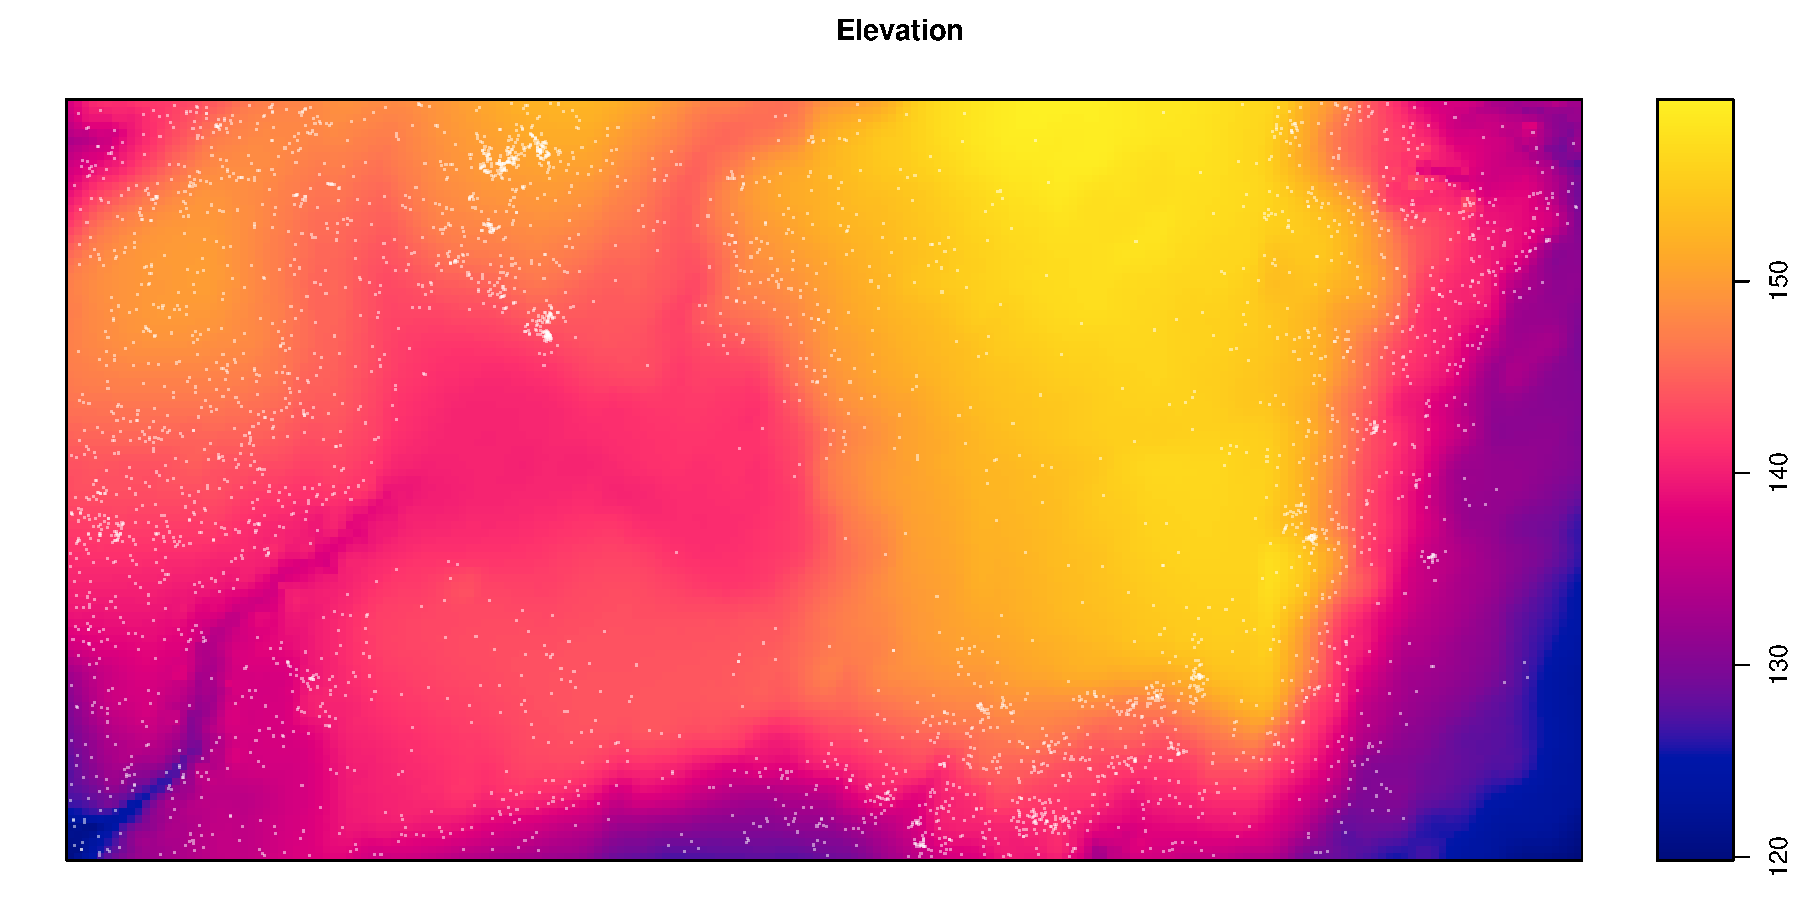
\includegraphics[width=0.9\textwidth]{figures/bei_elev.pdf}}

\subfloat[Magnitude of the elevation gradient, with events overlaid.]
{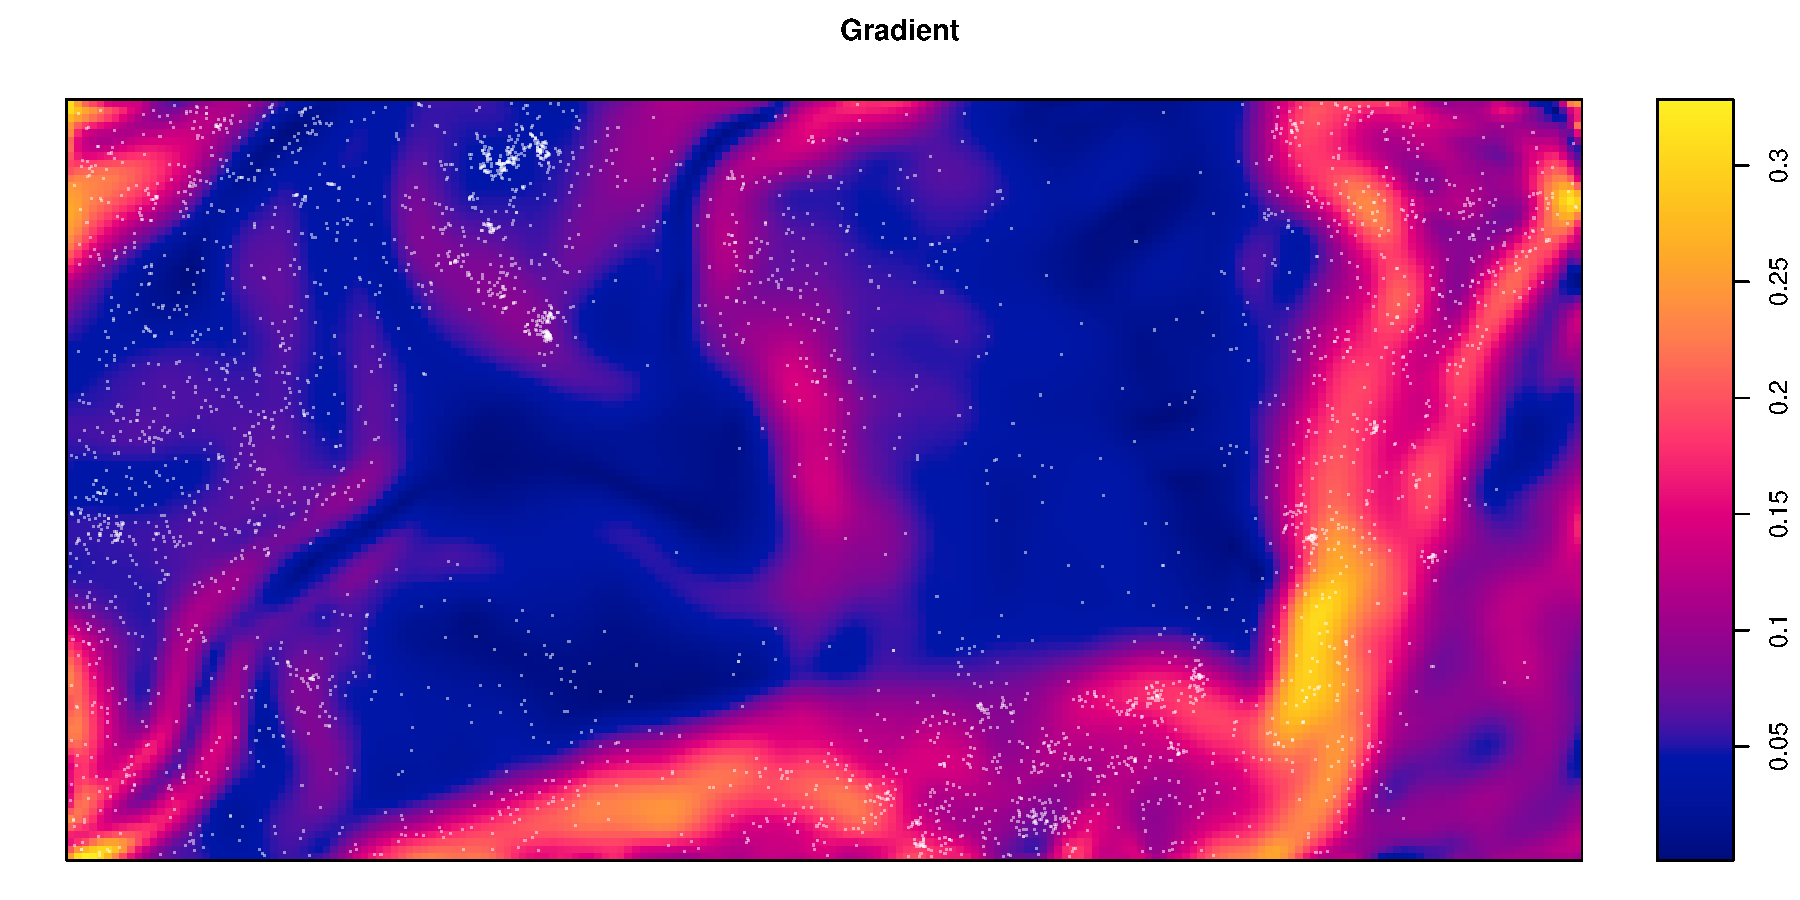
\includegraphics[width=0.9\textwidth]{figures/bei_grad.pdf}}

\caption{Plots of the event and covariate data for the \emph{Beilschmiedia
pendula Lauraceae} data analysis. The study region is 1000 m by 500 m.}
\label{bei}
\end{figure}

\subsection{Full {\it Beilschmiedia Pendula Lauraceae} Dataset}
\label{beianalysis}


\subsubsection{Model Specification}
\label{beimodel}

We use the log-Gaussian Cox process model with intensity
\begin{equation}
\log\left[\lambda(u)\right] = \beta_{0} + \beta_{1} z_{1}(u)
+ \beta_{2} z_{2}(u) + \mathbf{e}(u)
\end{equation}
where \(z_{1}(u)\) is the elevation at \(u\), \(z_{2}(u)\) is the magnitude of
the elevation gradient at \(u\), and \(\mathbf{e}(u)\) is a zero-mean
stationary and isotropic Gaussian process with Mat\'{e}rn covariance and fixed
\(\alpha = 2\). We parameterize the GP in terms of the standard deviation
\(\sigma\) and effective range \(\rho\). To connect this with the notation
from Section \ref{inla}, \(\boldsymbol{\theta} = (\sigma, \rho)'\) and
\(\boldsymbol{\xi} = (\beta_{0}, \beta_{1}, \beta_{2}, \mathbf{e}(s_{1}),
\dots, \mathbf{e}(s_{m}))'\).

The prior distributions are set as follows. \(\beta_{0}\), \(\beta_{1}\), and
\(\beta_{2}\) are independent \(\mathrm{N}(0, \infty)\). For the Mat\'{e}rn
covariance parameters, R-INLA provides a penalized complexity (PC) prior
defined in terms of the standard deviation \(\sigma\) and the effective range
\(\rho\) \cite{fuglstadetal,simpsonpc}. The PC prior is intended to provide an
intuitive way to define informative priors and is specified by defining a tail
probability for each parameter. R-INLA actually uses these inputs to set an
exponential prior on the precision \(\tau = 1 / \sigma^{2}\) and a Weibull
prior on the scale \(\kappa = \sqrt{8 \nu} / \rho\), but all of the software output
is provided in terms of \(\sigma\) and \(\rho\). We set
\(\mathrm{Pr}(\sigma > 2) = 0.1\) to be relatively uninformative for the SD of
a log-scale random effect, and \(\mathrm{Pr}(\rho < 5) = 0.1\) similar to the
prior used by M\"{o}ller and Waagepetersen~\cite{moellerwaagepetersen}.


\subsubsection{Fitting in R-INLA}
\label{beifitting}

We fit the model using R-INLA package and its implementation of
the SPDE approach. Some manual preprocessing was needed to employ the Poisson
factorization. Our R code can be found in the supplementary materials. This
section provides a conceptual explanation of the model-fitting process.

The first task is to construct a mesh for the piecewise linear approximations.
A 25 meter resolution appears adequate to accurately represent the covariate
surfaces. We used tools in R-INLA to create a Delaunay
triangulation with a maximum edge length of 25~m. The resulting mesh has
\(m = 2145\) nodes \(s_{1},  \dots, s_{2145}\) and 4096
triangles~(Figure~\ref{beimesh}). We used linear interpolation to approximate
the covariates \(z_{1}(s_{i})\) and \(z_{2}(s_{i})\) at each node. After
creating the mesh, we specify the priors for the covariance parameters and
R-INLA initializes an object to represent the covariance structure
on the mesh.

\begin{figure}[t!]\centering
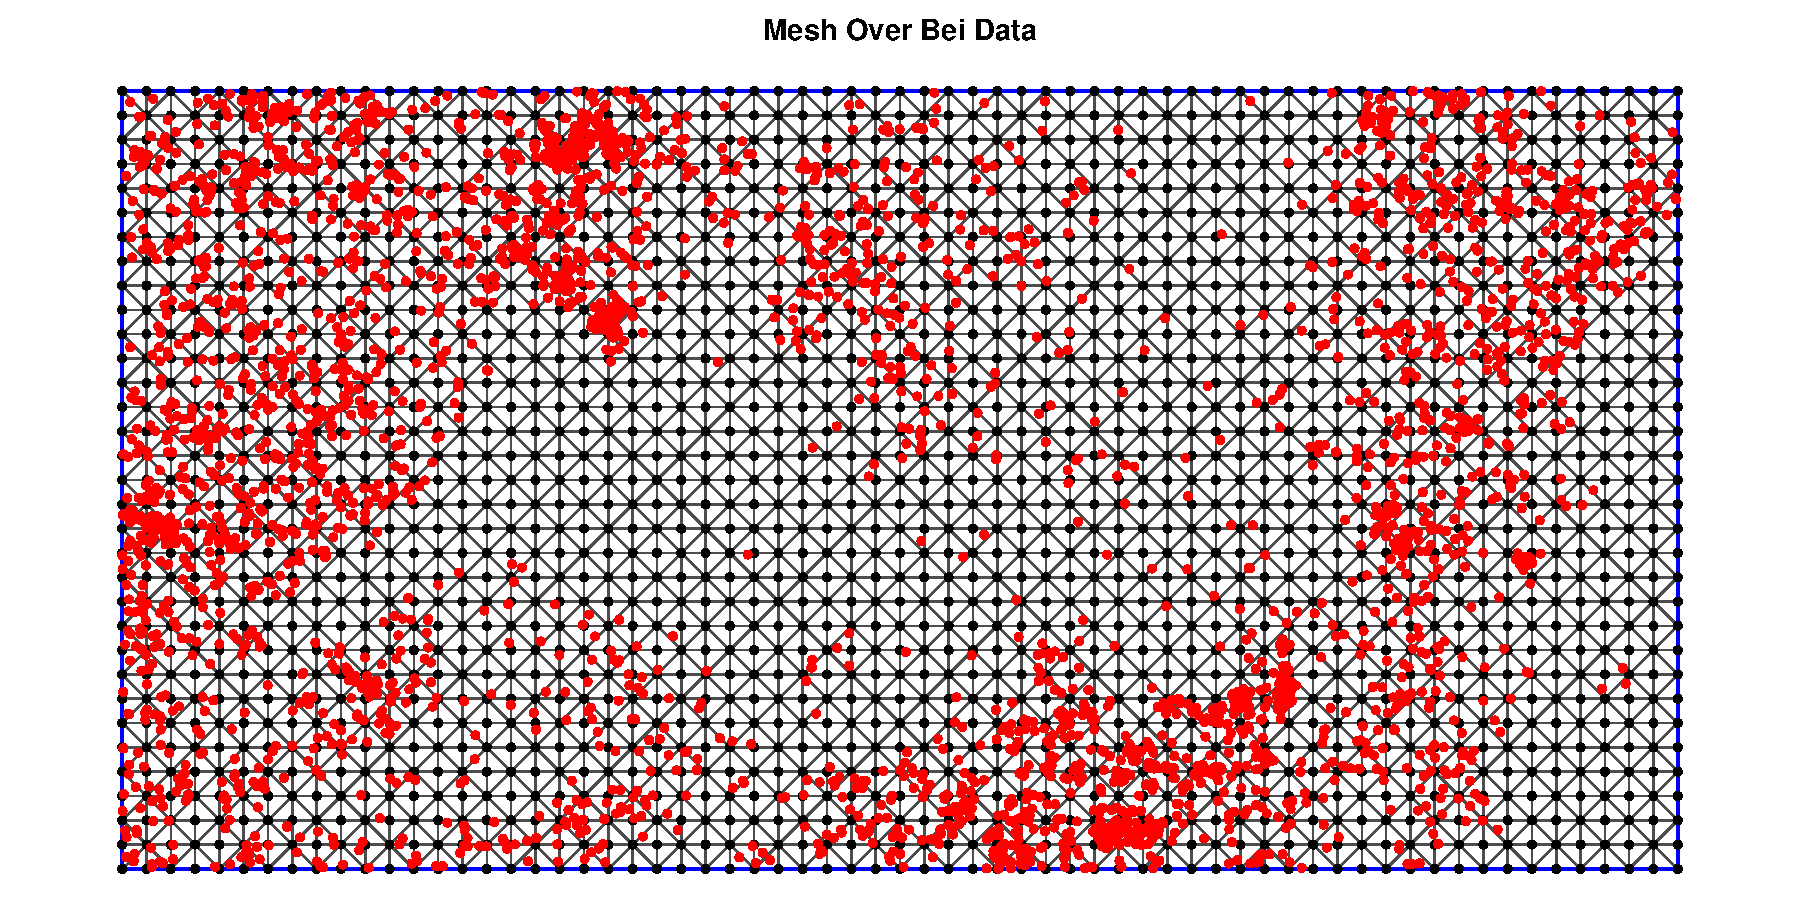
\includegraphics[width=\textwidth]{figures/bei_mesh.pdf}
\caption{Triangular mesh with pseudodata overlaid for the \emph{Beilschmiedia
pendula Lauraceae} data analysis. Black dots represent pseudodata with values
of 0 at the mesh nodes. Red dots represent pseudodata with values of 1 at the
events.}
\label{beimesh}
\end{figure}

The next step is to define the pseudodata, find the barycentric coordinate
matrix \(\mathbf{A}\), and calculate the numerical integration weights. The
pseudodata vector is
\begin{equation}
\mathbf{y} = (0, \dots, 0, 1, \dots, 1)'
\end{equation}
consisting of 2145 zeros corresponding to the mesh nodes and 3604 ones
representing the events. The first 2145 rows of \(\mathbf{A}\) are an
identity matrix; the remaining rows are the barycentric coordinates of the
events, which R-INLA calculates for us. The weight vector is
\begin{equation}
\boldsymbol{\alpha} = (\alpha_{1}, \dots, \alpha_{2145}, 0, \dots, 0)'.
\end{equation}
The alphas equal one-third of the total area of all triangles of which each
node is a vertex, calculated by R-INLA. The zeros correspond to the
3604 events, which do not contribute to the numerical integration.

The final bit of setup is to combine the pseudodata, covariates at the nodes,
and a vector of node indices into a data list for the \texttt{inla()} function.
This function is then called with arguments specifying a formula for the
linear predictor, a Poisson family model (which defaults to a log link), the
data list, the \(\mathbf{A}\) matrix, the priors for the coefficients, and the
\(\boldsymbol{\alpha}\) vector as the exposure parameter. This function
delivers the posterior marginal distribution of each parameter, latent
variable, and any requested linear combinations of those. The \texttt{inla()} function takes about 90 seconds to fit the model on a midrange laptop. It is worth noting that joint samples can also be taken using \texttt{inla.posterior.sample()} which uses a Monte Carlo procedure to sample from the internal joint mixture approximation.

\subsubsection{Results}
\label{beiresults}

\begin{figure}[t!]\centering

\subfloat[Posterior mean surface for the fixed effects.]
{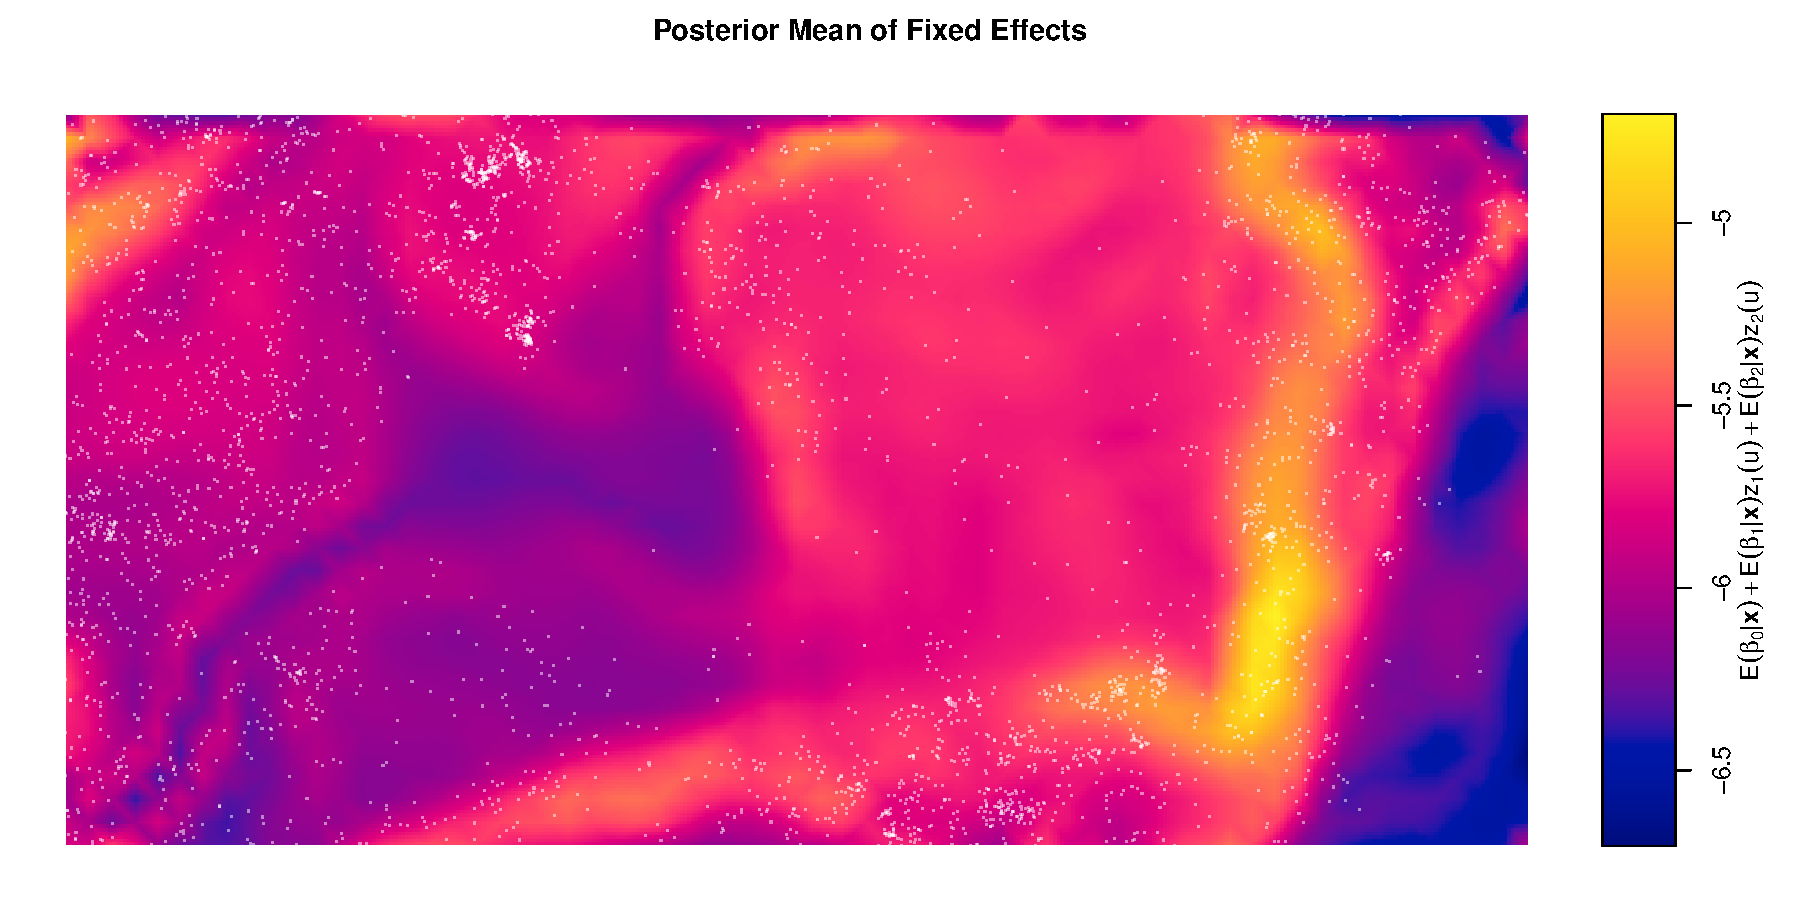
\includegraphics[width=0.9\textwidth]{figures/bei_betas.pdf}}

\subfloat[Posterior mean of the GP prediction surface.]
{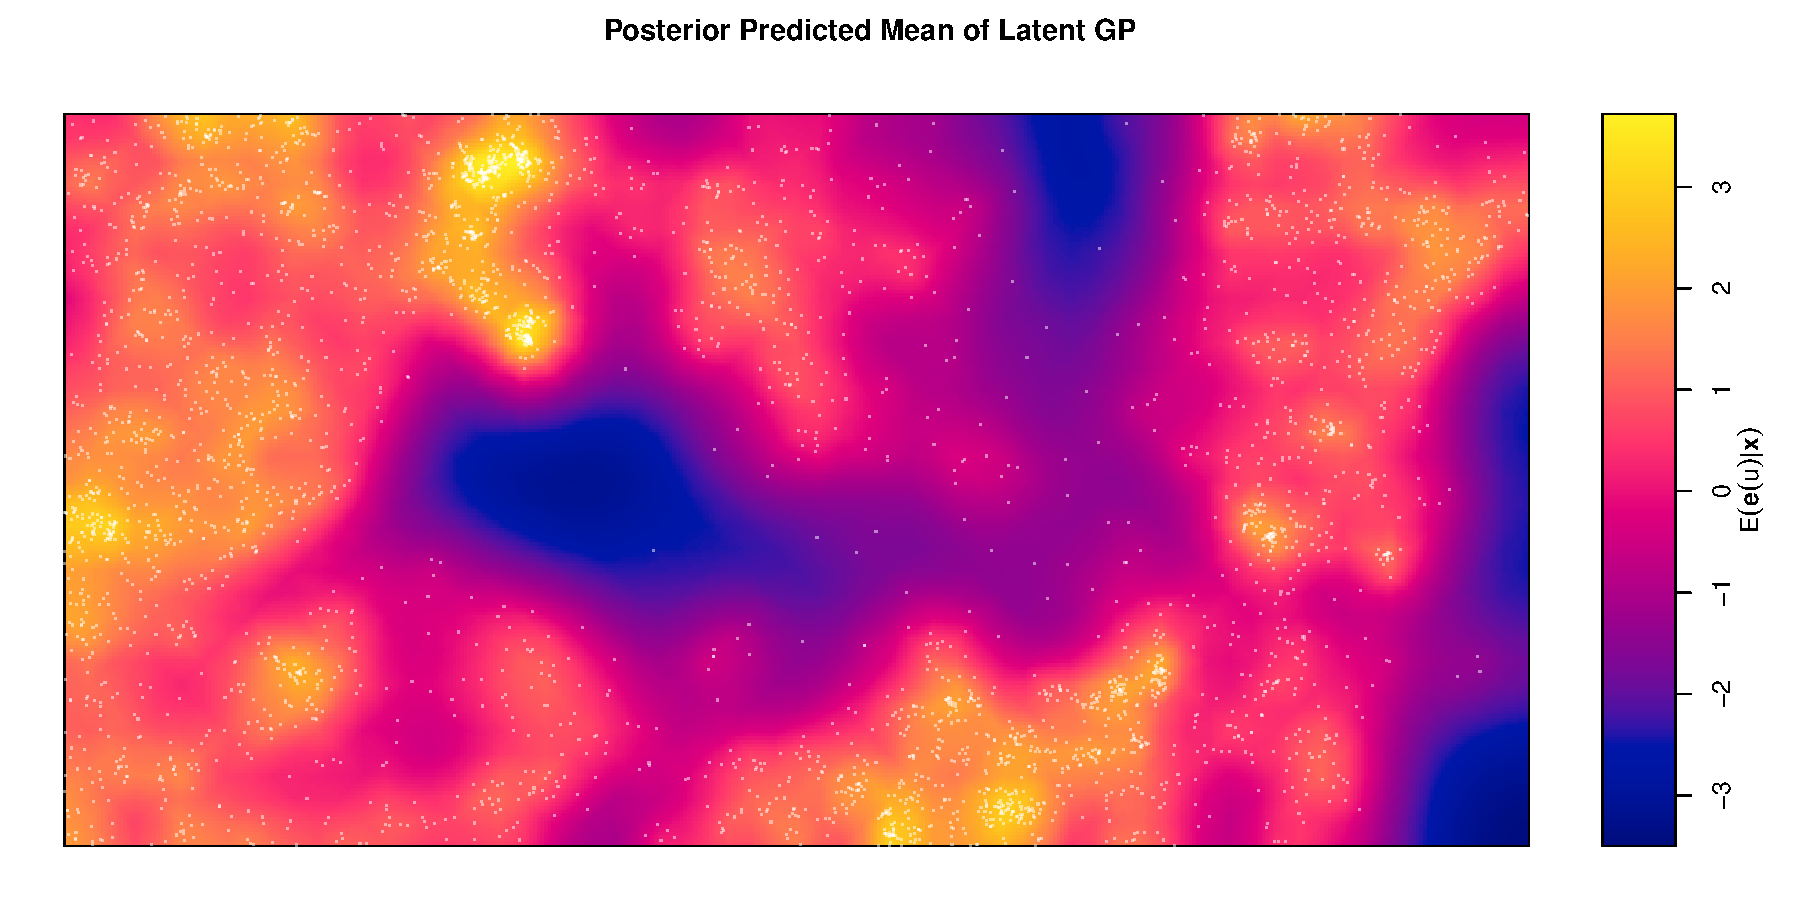
\includegraphics[width=0.9\textwidth]{figures/bei_mean.pdf}}

\caption{Posterior mean surfaces of the fixed effects component and the
spatial GP from the \emph{Beilschmiedia pendula Lauraceae} data analysis.}
\label{beimean}
\end{figure}

The posterior marginals provide evidence that both higher elevation and larger
gradient are associated with higher intensity. The elevation coefficent
\(\beta_{1}\) has a posterior mean of 0.0328 with a central 95\% interval of
\((0.0112, 0.0547)\), and the gradient coefficient \(\beta_{2}\) has posterior
mean 4.44 with 95\% interval \((2.42, 6.46)\). The posterior mean of the
intercept \(\beta_{0}\) is \(-10.9\) with 95\% interval of \((-14.2, -7.63)\).
Mapped across space, the posterior mean of the fixed effect component of the
linear predictor
\begin{equation}
E(\beta_{0} | \mathbf{x}) + E(\beta_{1} | \mathbf{x}) z_{1}(u)
+ E(\beta_{2} | \mathbf{x}) z_{2}(u)
\end{equation}
appears as an average of the elevation and gradient
surfaces~(Figure~\ref{beimean},~top).

The fixed effects do not explain all of the heterogeneity of the point pattern;
some spatial structure remains to be described by the posterior predicted
GP~(Figure~\ref{beimean},~bottom). The prediction surface shows a large region
of low values in the center where there are nearly no events, and hotspots
where many events are clumped together. The GP standard deviation \(\sigma\)
has posterior mean 1.30 and 95\% central interval \((1.05, 1.63)\), while the
range parameter \(\rho\) has a posterior mean of 176 with a 95\% interval of
\((137, 229)\).


\subsubsection{Model Checking}
\label{beiresid}

\begin{figure}[t!]\centering

\subfloat[Posterior intensity surface in events per square meter, calculated
using the piecewise linear approximate covariate surfaces and the posterior
means of the intercept, coefficients, and GP.]
{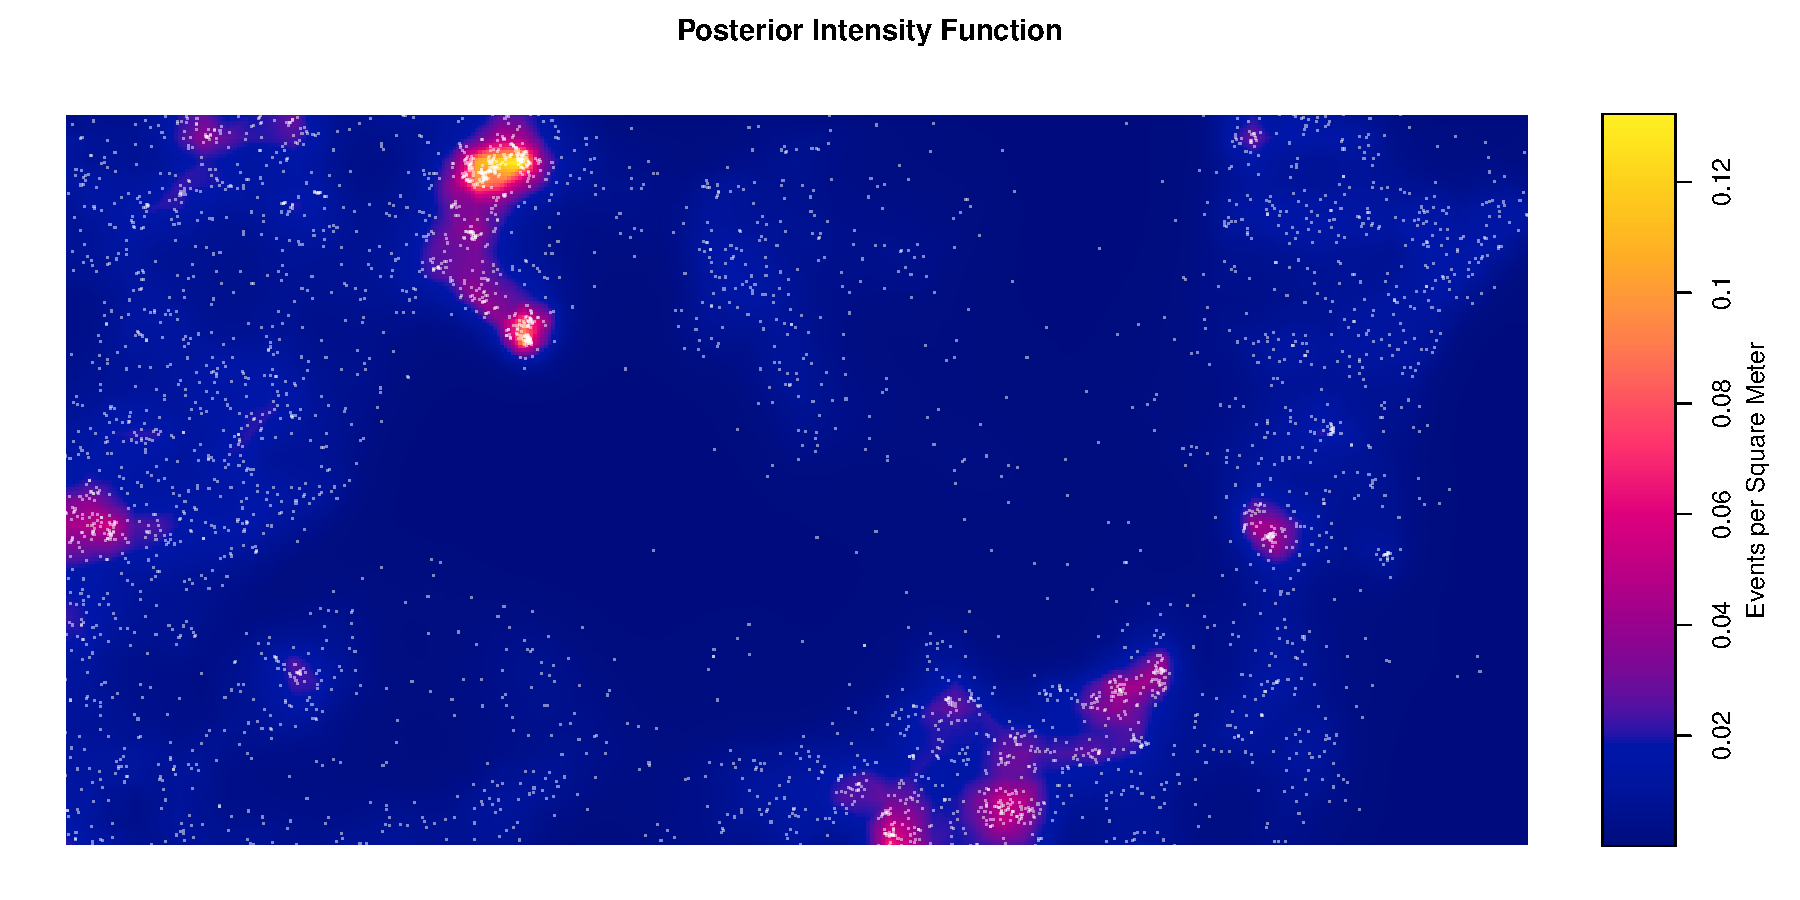
\includegraphics[width=0.9\textwidth]{figures/bei_intensity.pdf}}

\subfloat[Pearson residuals calculated on a grid.]
{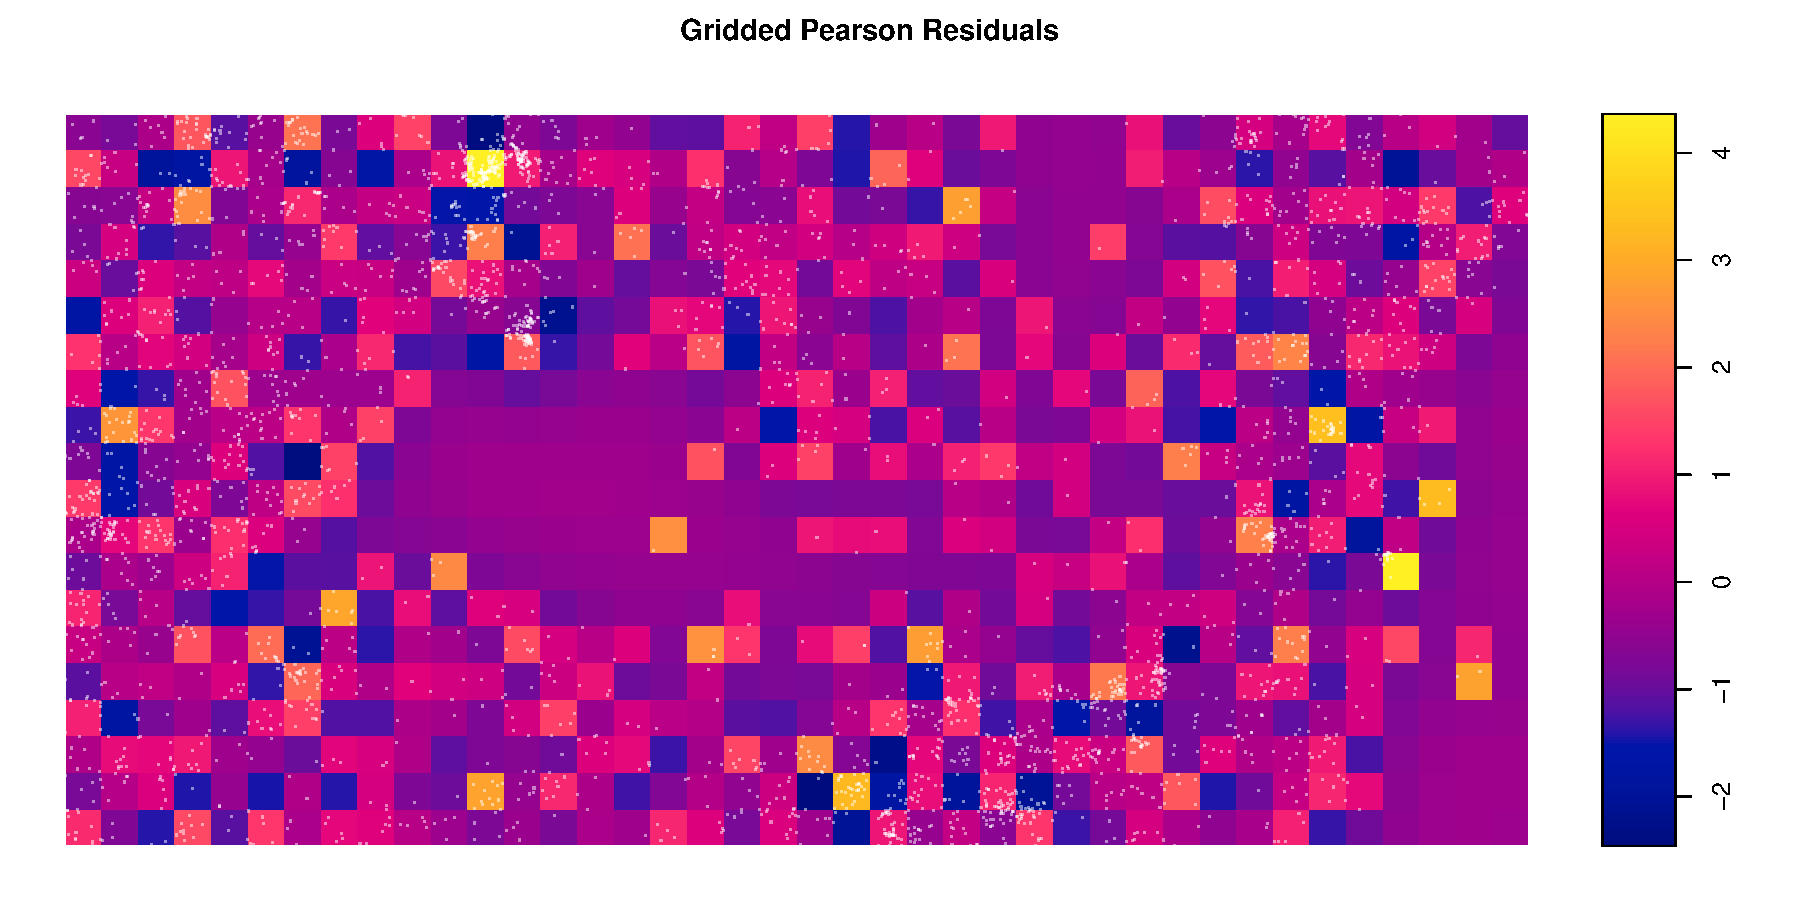
\includegraphics[width=0.9\textwidth]{figures/bei_residuals.pdf}}

\caption{Posterior mean intensity function and Pearson residuals calculated
using the posterior mean intensity from the \emph{Beilschmiedia pendula
Lauraceae} data analysis.}
\label{beiintensity}
\end{figure}

This section provides a brief and simple residual analysis to illustrate that
their are no glaring issues with the model fit. Literature on residual analysis
for spatial point process models is quite rich and not specific to INLA; for a
more general discussion see Baddeley et. al.~(2005)~\cite{baddeleyresiduals}.

We calculated the Pearson residuals
\begin{equation}
\frac{\text{Observed count} - \text{Expected count}}
{\sqrt{\text{Expected count}}}
\end{equation}
on a 40 by 20 lattice of grid cells. We used functions from R-INLA to transform
predictions from the log-scale to the natural scale and calculate the posterior
mean intensity at the center of each grid
cell~(Figure~\ref{beiintensity},~top). The expected counts were approximated by the posterior mean intensity times the area of the grid cell. The bottom panel
of Figure~\ref{beiintensity} shows the Pearson residuals mapped across space.

The residuals have small magnitude in the central region and on the eastern
edge where there are no observed events and low mean posterior intensity. This
is not surprising because it is not possible to see much variation in counts
in that region. There are a few large-magnitude positive residuals (about 4)
suggesting there is some clustering not described by the model. Elsewhere, the
residuals appear random with no obvious spatial patterns. We repeated the
residual analysis with several grid cell sizes and saw the same characteristics
each time.


\subsection{Transect Sampling Example}
\label{xsectanalysis}

\begin{figure}[p!]\centering

\subfloat[Locations of observed trees (events).]
{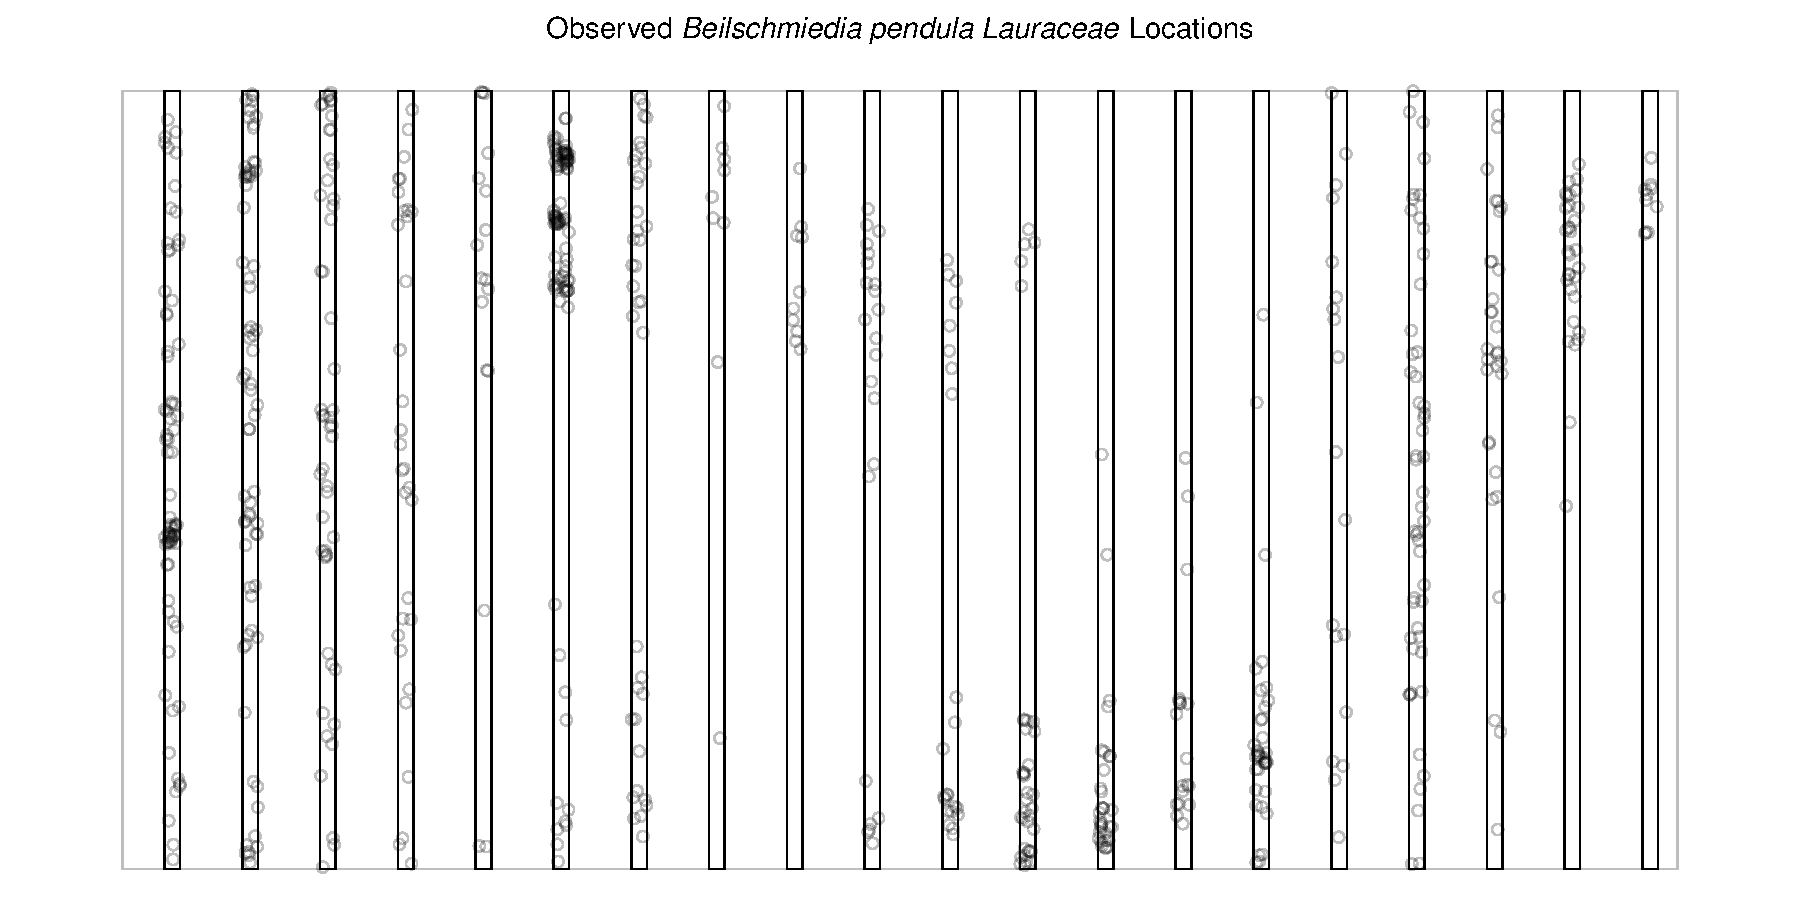
\includegraphics[width=0.9\textwidth]{figures/bei-effort.pdf}}

\subfloat[Elevation in meters, with observed region and events overlaid.]
{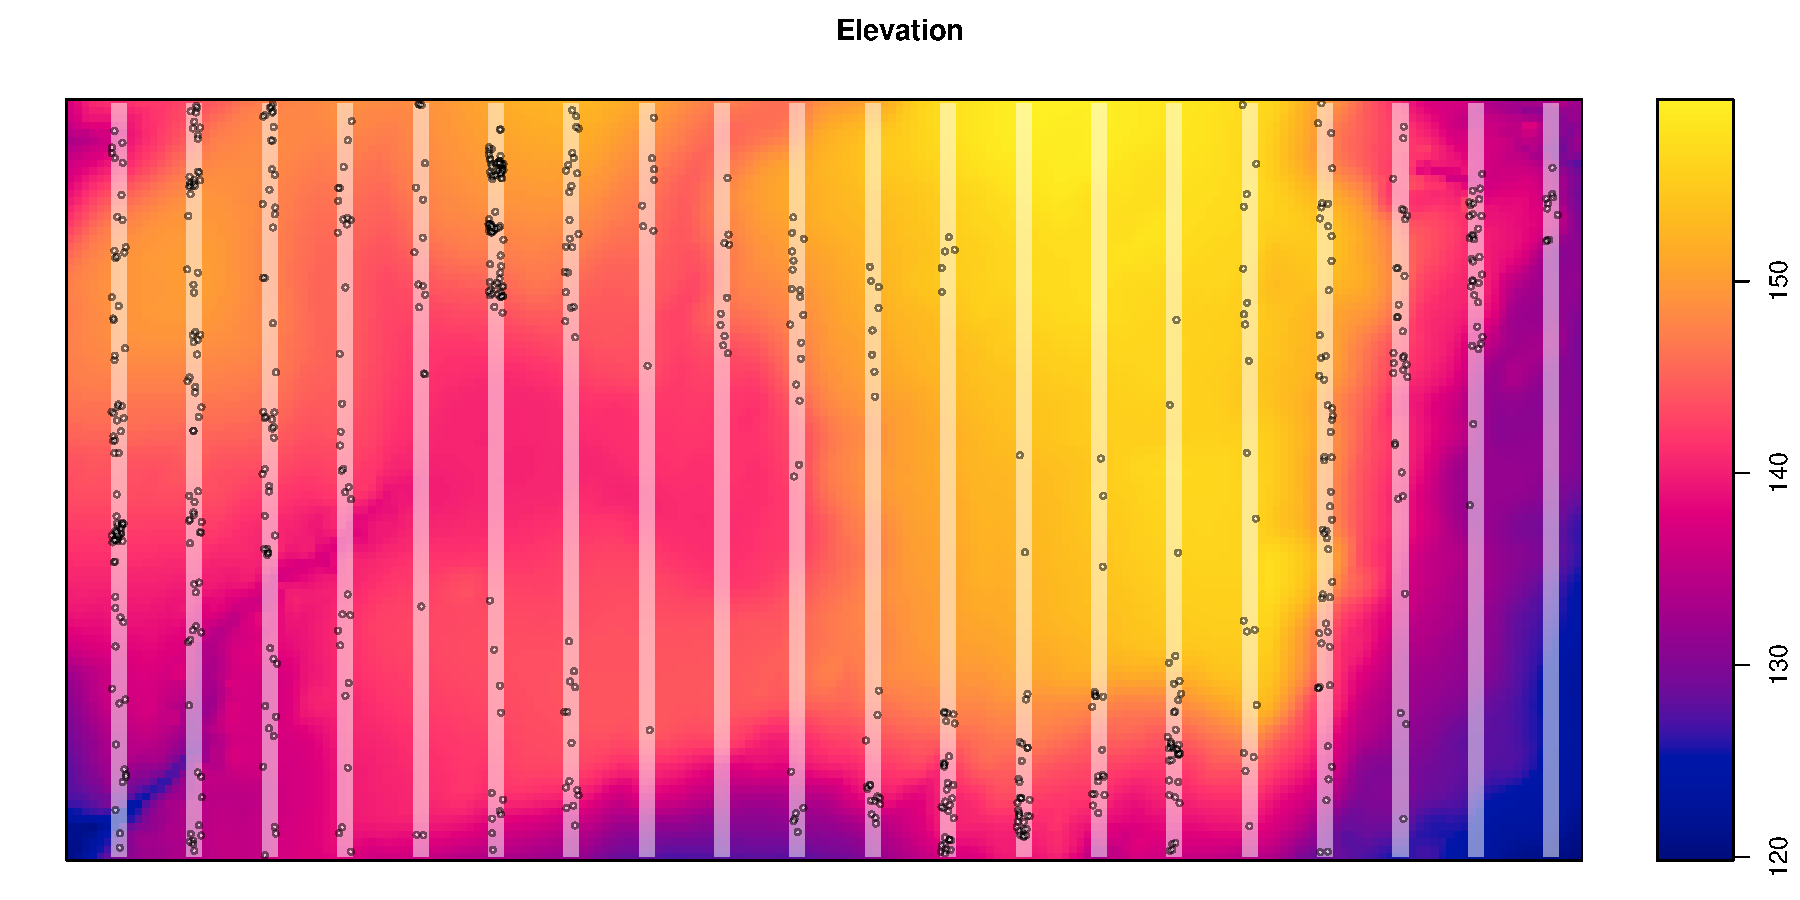
\includegraphics[width=0.9\textwidth]{figures/bei-effort_elev.pdf}}

\subfloat[Magnitude of the elevation gradient, with observed region and events
overlaid.]
{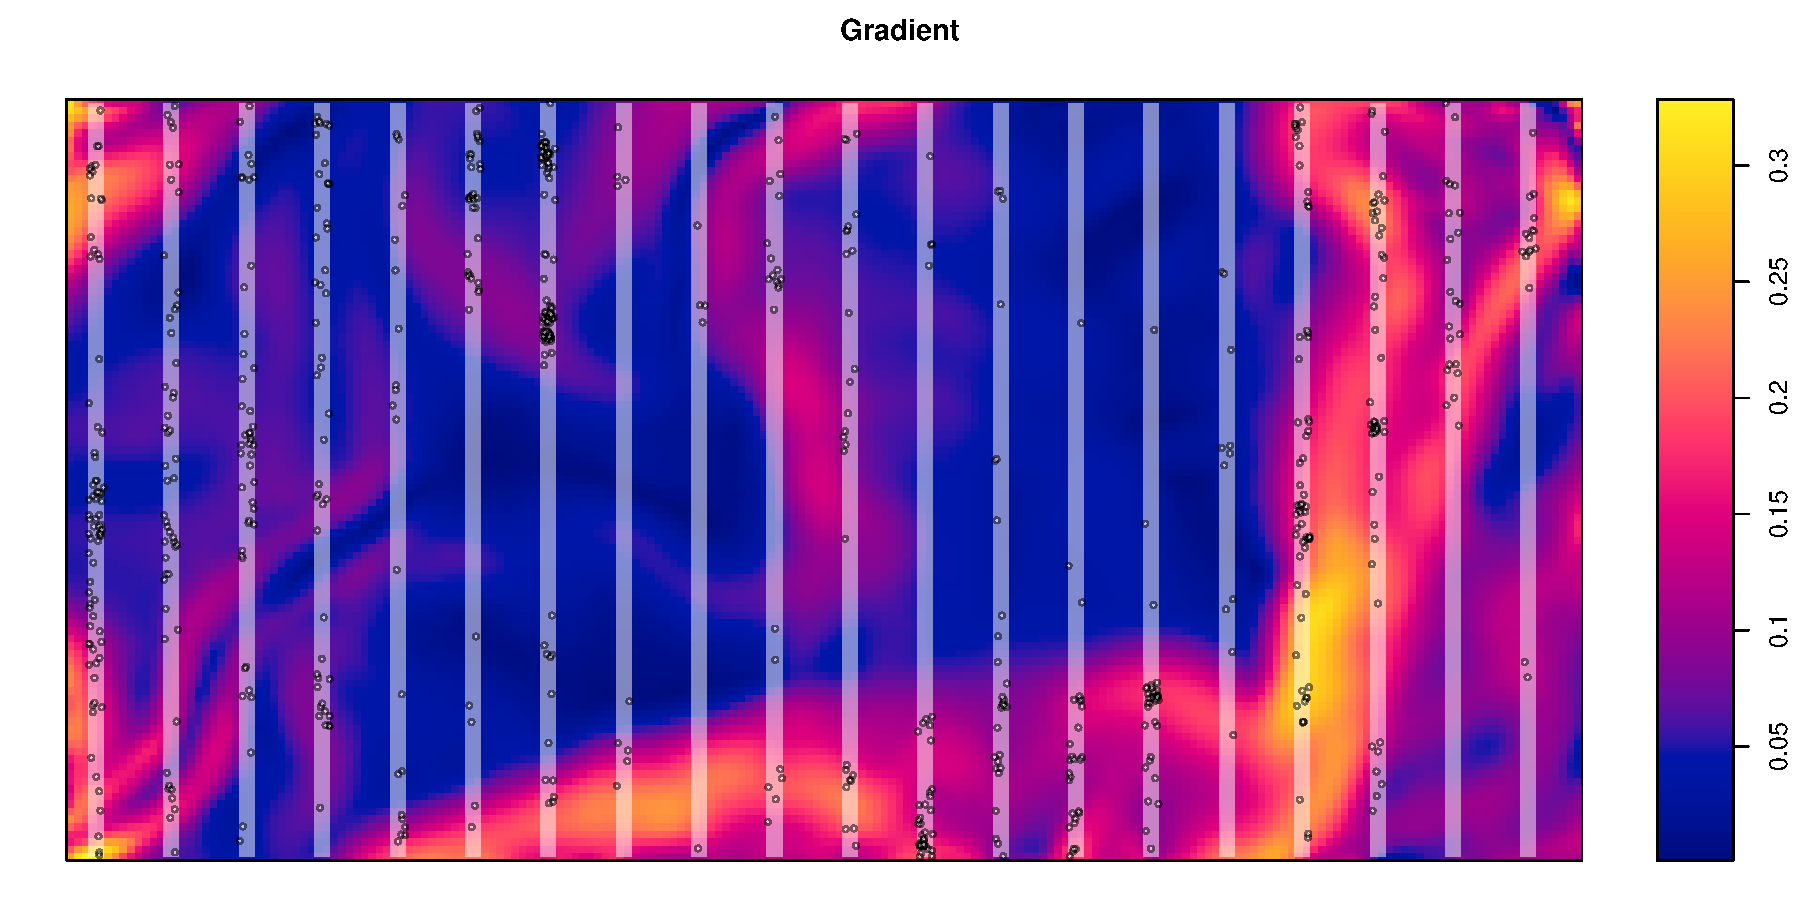
\includegraphics[width=0.9\textwidth]{figures/bei-effort_grad.pdf}}

\caption{Plots of the event and covariate data for the simulated transect
survey. The study region is 1000 m by 500 m.}
\label{effort}
\end{figure}

In this section, we illustrate the analysis of incompletely-observed point
pattern data using the \emph{Beilschmiedia pendula Lauraceae} and a simulated
transect sampling scheme. The example uses a survey scheme where all events in
a subset of the study region are recorded. This type of variable sampling
effort requires more programming effort than distance sampling, and the
difference is worth explaining. We also provide R code for a distance sampling
example in the supplementary materials, but the preprocessing and model-fitting
procedure for distance sampling data is not much more complicated than for the
fully-observed case.

Suppose part of the study requires every observed tree to be visited so
time-consuming measurements can be made on each. For practical reasons, the
researchers decide to take a systematic sample of transects and limit data
collection to events within 5~m of a transect. Sections of the site farther
than 5~m from a transect are unobserved, meaning events in those regions
cannot be observed and nothing is known about the number of events or their
locations. We assume the elevation and gradient data were available from
another source so that the full covariate data can be used to predict the
intensity in the unobserved parts of the site.

We simulate this by choosing a random starting point and defining transects
running north-south spaced 50~m apart. All events within 5~m of a transect are
saved; all other events are discarded. The result is \(n = 710\) events
observed in 20 rectangles sized 500~m by 10~m~(Figure~\ref{effort}).


\subsubsection{Model Specification}
\label{xsectmodel}

We use the same model as fit to the full data, a log-Gaussian Cox process model
with intensity
\begin{equation}
\log\left[\lambda(u)\right] = \beta_{0} + \beta_{1} z_{1}(u)
+ \beta_{2} z_{2}(u) + \mathbf{e}(u).
\end{equation}
As before, \(z_{1}(u)\) is the elevation at \(u\), \(z_{2}(u)\) is the
magnitude of the elevation gradient at \(u\), and \(\mathbf{e}(u)\) is a
zero-mean Gaussian process with Mat\'{e}rn covariance and \(\alpha = 2\).
The prior distributions are again \(\beta_{0}\), \(\beta_{1}\), and
\(\beta_{2}\) independent \(\mathrm{N}(0, \infty)\),
\(\mathrm{Pr}(\sigma > 2) = 0.1\), and \(\mathrm{Pr}(\rho < 5) = 0.1\).


\subsubsection{Fitting in R-INLA}
\label{xsectfitting}

\begin{figure}[p!]
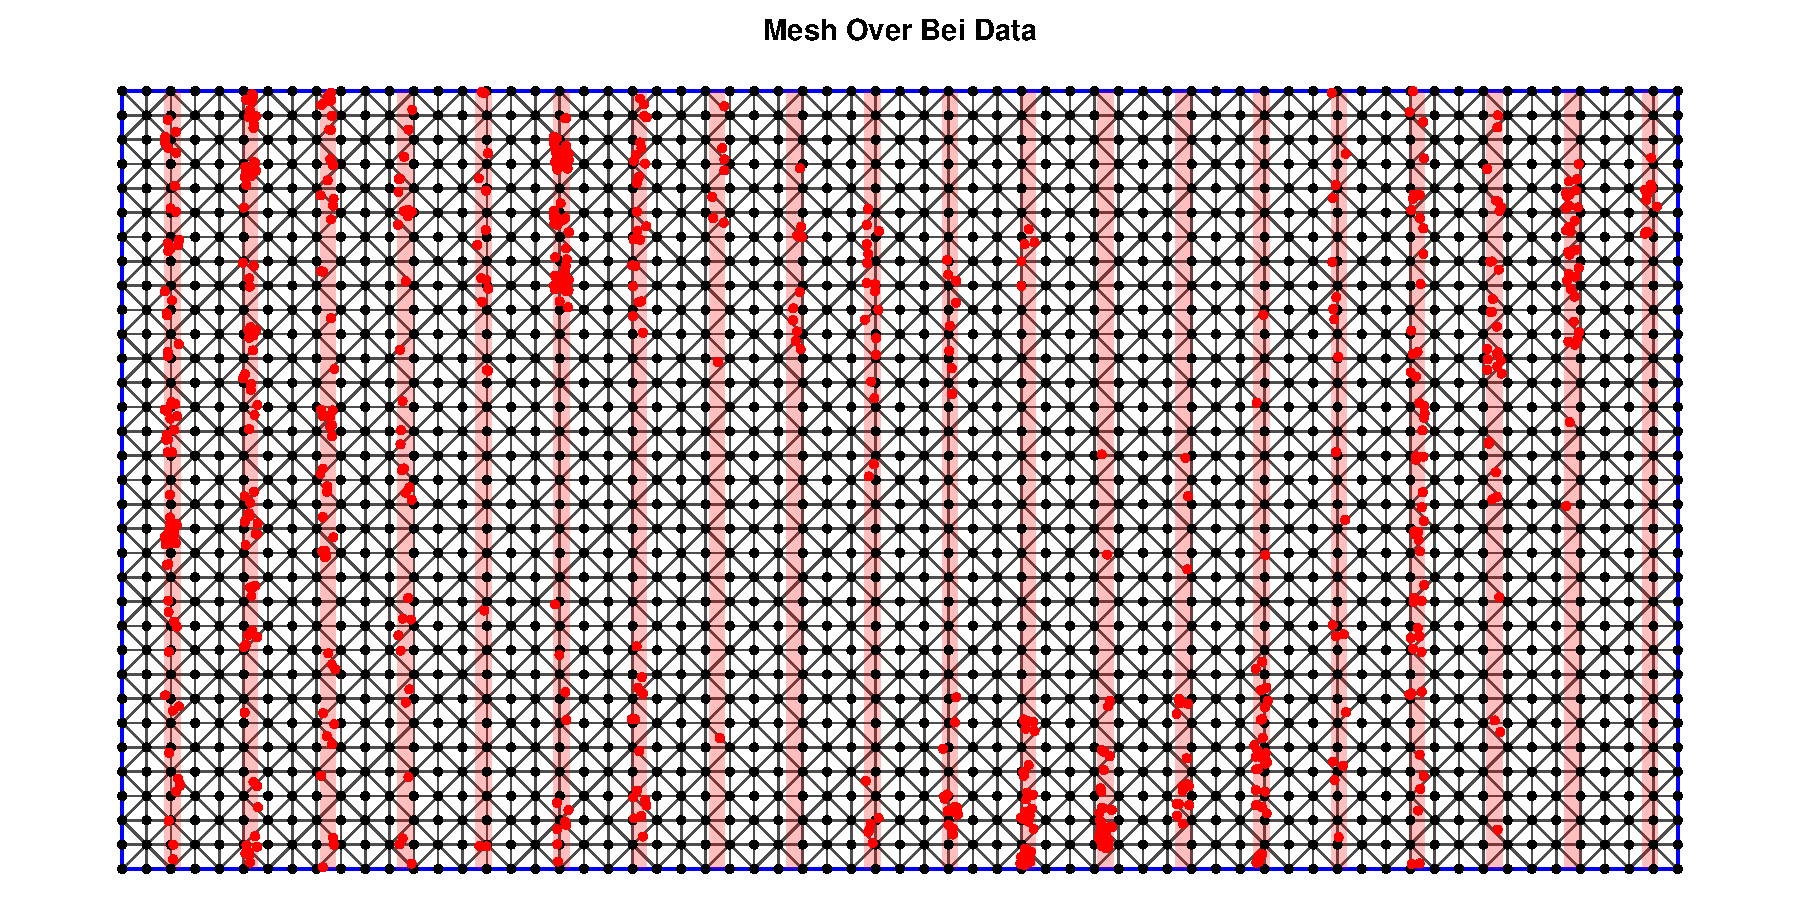
\includegraphics[width=\textwidth]{figures/bei-effort_mesh.pdf}
\caption{Triangular mesh with observed region and events overlaid for the
simulated transect data analysis. Black dots represent pseudodata with values
of 0 at the mesh nodes. Red dots represent pseudodata with values of 1 at the
observed events.}
\label{effortmesh}
\end{figure}

\begin{figure}[p!]
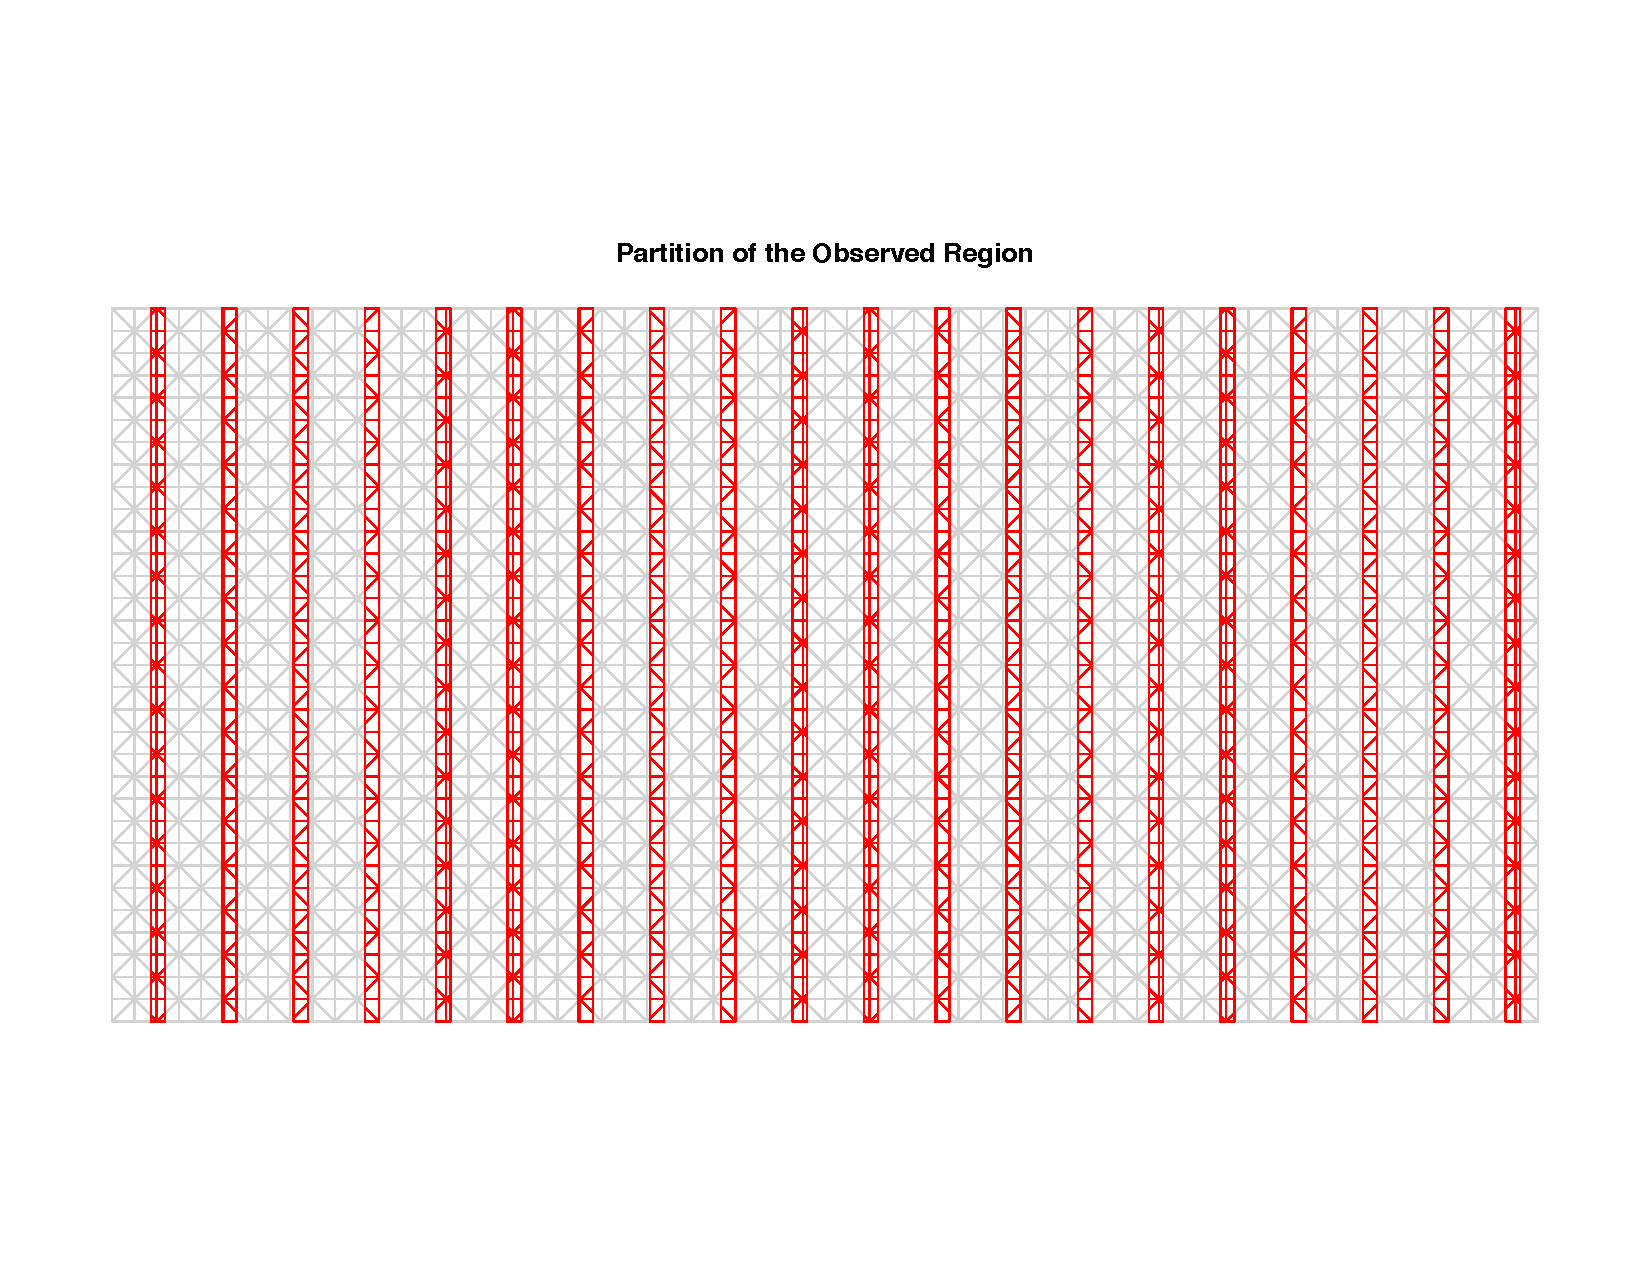
\includegraphics[width=\textwidth]{figures/bei-effort_partition.pdf}
\caption{Partition of the observed region created by intersection with each
mesh triangle.}
\label{effortpartition}
\end{figure}

The procedure for fitting the LGCP model to variable sampling effort data is
the same as for fully-observed data except that the weight vector
\(\boldsymbol{\alpha}\) is different. Our code is available in the
supplementary materials.

The mesh~(Figure~\ref{effortmesh}) is the same as used with the fully-observed
point pattern, with \(m = 2145\) nodes. We interpolated the covariates
at the nodes and had R-INLA initialize the covariance structure as
before. The pseudodata vector changes dimension, becoming
\begin{equation}
\mathbf{y} = (0, \dots, 0, 1, \dots, 1)'
\end{equation}
with 2145 zeros corresponding to the mesh nodes and 710 ones for the observed
events.

The computation of the weight vector is more involved. The notation is again
\begin{equation}
\boldsymbol{\alpha} = (\alpha_{1}, \dots, \alpha_{2145}, 0, \dots, 0)',
\end{equation}
now with 710 zeros representing the observed events. The alphas equal the
observed area represented by each node. We used tools from \texttt{spatstat}
to calculate these areas. First, we created an \texttt{owin} object defining
the observed region along the transects. Then, we created a list of
\texttt{owin} objects with each representing one triangle of the mesh. Next,
we intersected the observed region with each triangle to partition the observed
region into many small shards, each contained within a single
triangle~(Figure~\ref{effortpartition}). Then we calculated the area of each
shard. These areas are each associated with a triangle, but the need to be
allocated to the nodes at the vertices of the triangle. To do this, we found
the centroid of each shard and allocated the area proportional to the
barycentric coordinates of the centroid. This way, the area of each shard is
distributed to the three nodes which define the triangle, and the closest node
gets the most weight while the farthest node get the least weight. Finally,
the alpha value for each node is computed by summing the weights contributed
by each shard to that node.

Finally, the pseudodata, covariates, and a node index are combined into a data
list and the \texttt{inla()} function is called to fit the model. The model
takes about 65 seconds to fit on our laptop computer.


\subsubsection{Results}
\label{xsectresults}

The fixed effect posterior marginals give evidence of relationships between
the intensity and both elevation and gradient. The elevation coefficient
\(\beta_{1}\) has a posterior mean of 0.0444 and a central 95\% posterior
interval of \((0.00686, 0.0836)\). The gradient coefficient \(\beta_{2}\) has
a posterior mean of 6.21 and a 95\% interval of \((3.24, 9.20)\). The
intercept \(\beta_{0}\) has posterior mean \(-12.7\) and 95\% interval
\((-18.6, -7.10)\). The posterior mean of the fixed effect component of the
linear predictor again appears as an average of the elevation and gradient
surfaces~(Figure~\ref{effortmean},~top), very similar to the previous figure.

As before, there is some additional spatial structure described by the
GP~(Figure~\ref{effortmean},~bottom). The prediction surface has low values
in the center and north where no events were observed, hotspots where events
are concentrated along the transects, and smooth transitions across the
unsurveyed regions between transects. The standard deviation \(\sigma\) has a
posterior mean of 1.27 with a central 95\% posterior interval of
\((0.956, 1.70)\). The range \(\rho\) has a posterior mean of 232 and
95\% interval of \((161, 340)\).

\begin{figure}[t!]\centering

\subfloat[Posterior mean surface for the fixed effects.]
{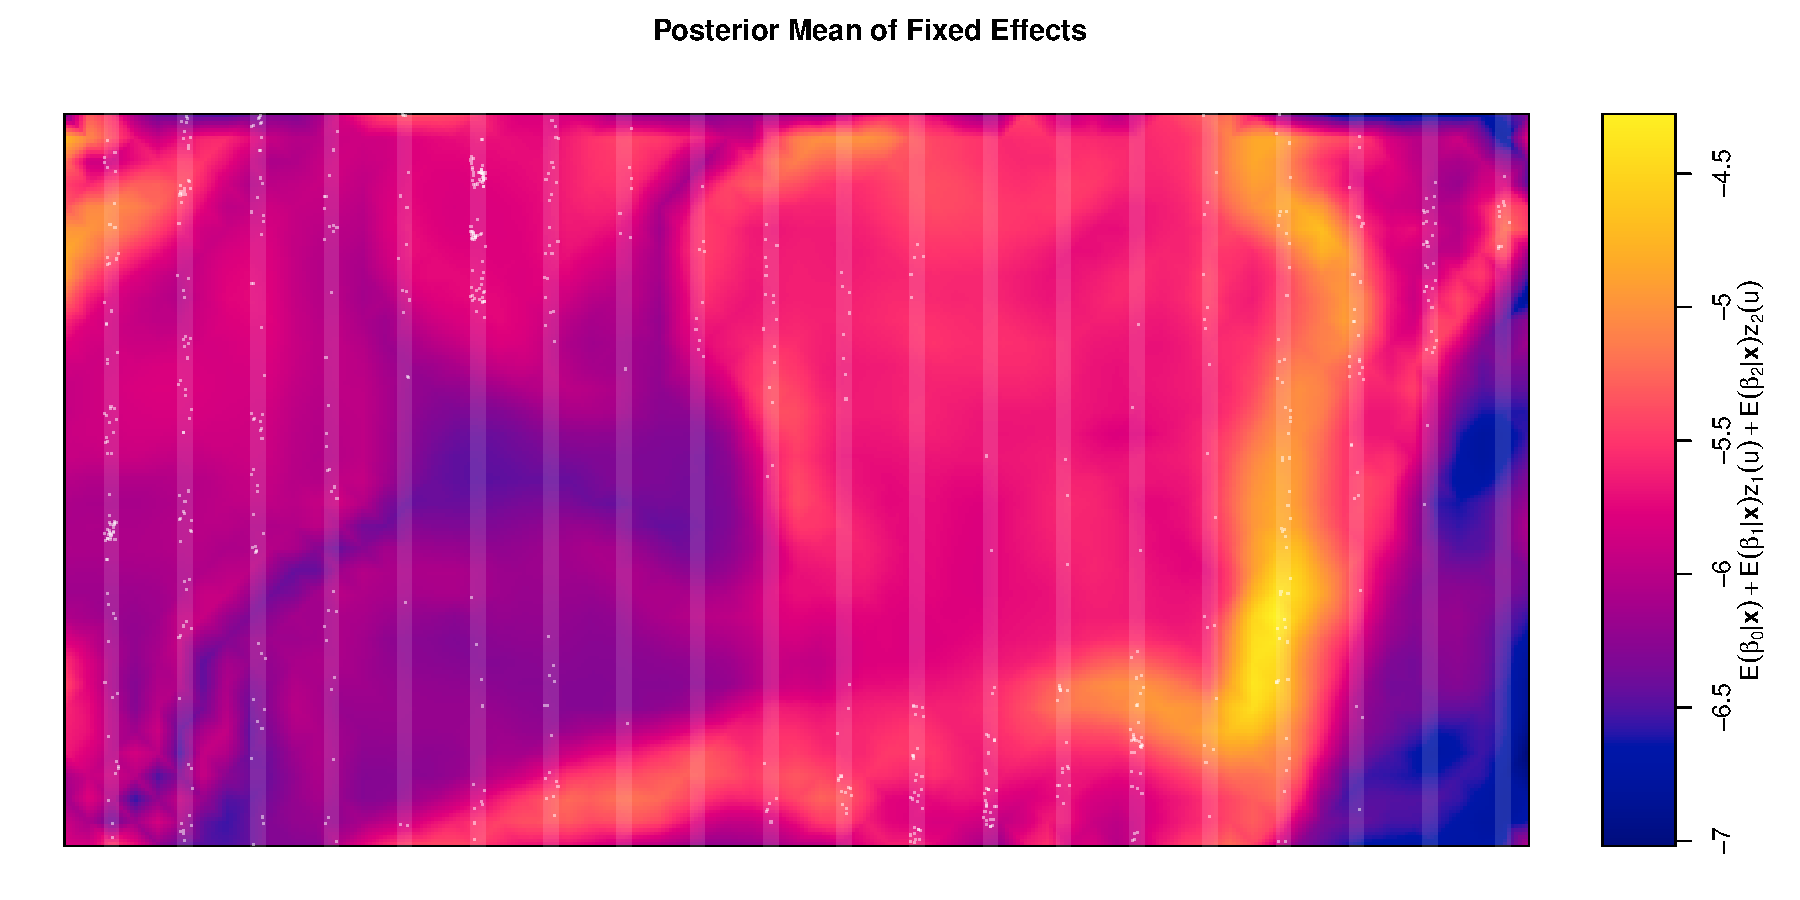
\includegraphics[width=0.9\textwidth]{figures/bei-effort_betas.pdf}}

\subfloat[Posterior mean of the GP prediction surface.]
{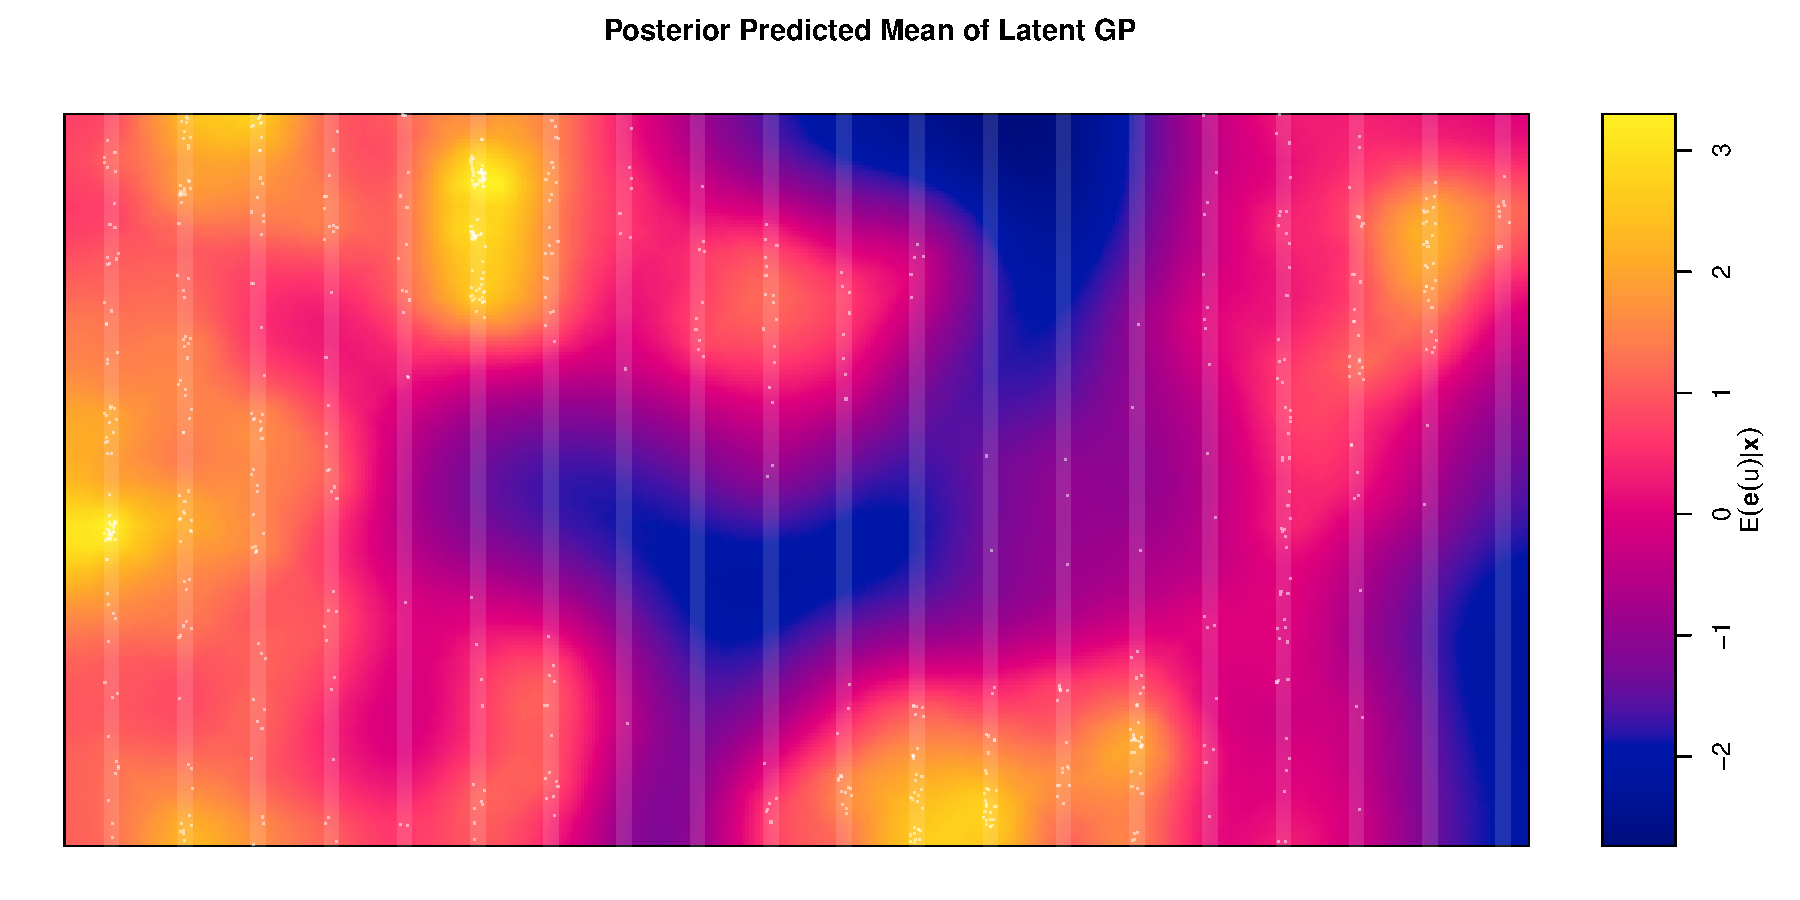
\includegraphics[width=0.9\textwidth]{figures/bei-effort_mean.pdf}}

\caption{Posterior mean surfaces of the fixed effects component and the
spatial GP from the simulated transect data analysis.}
\label{effortmean}
\end{figure}

\begin{figure}[t!]\centering

\subfloat[Posterior intensity surface in events per square meter, calculated
using the piecewise linear approximate covariate surfaces and the posterior
means of the intercept, coefficients, and GP.]
{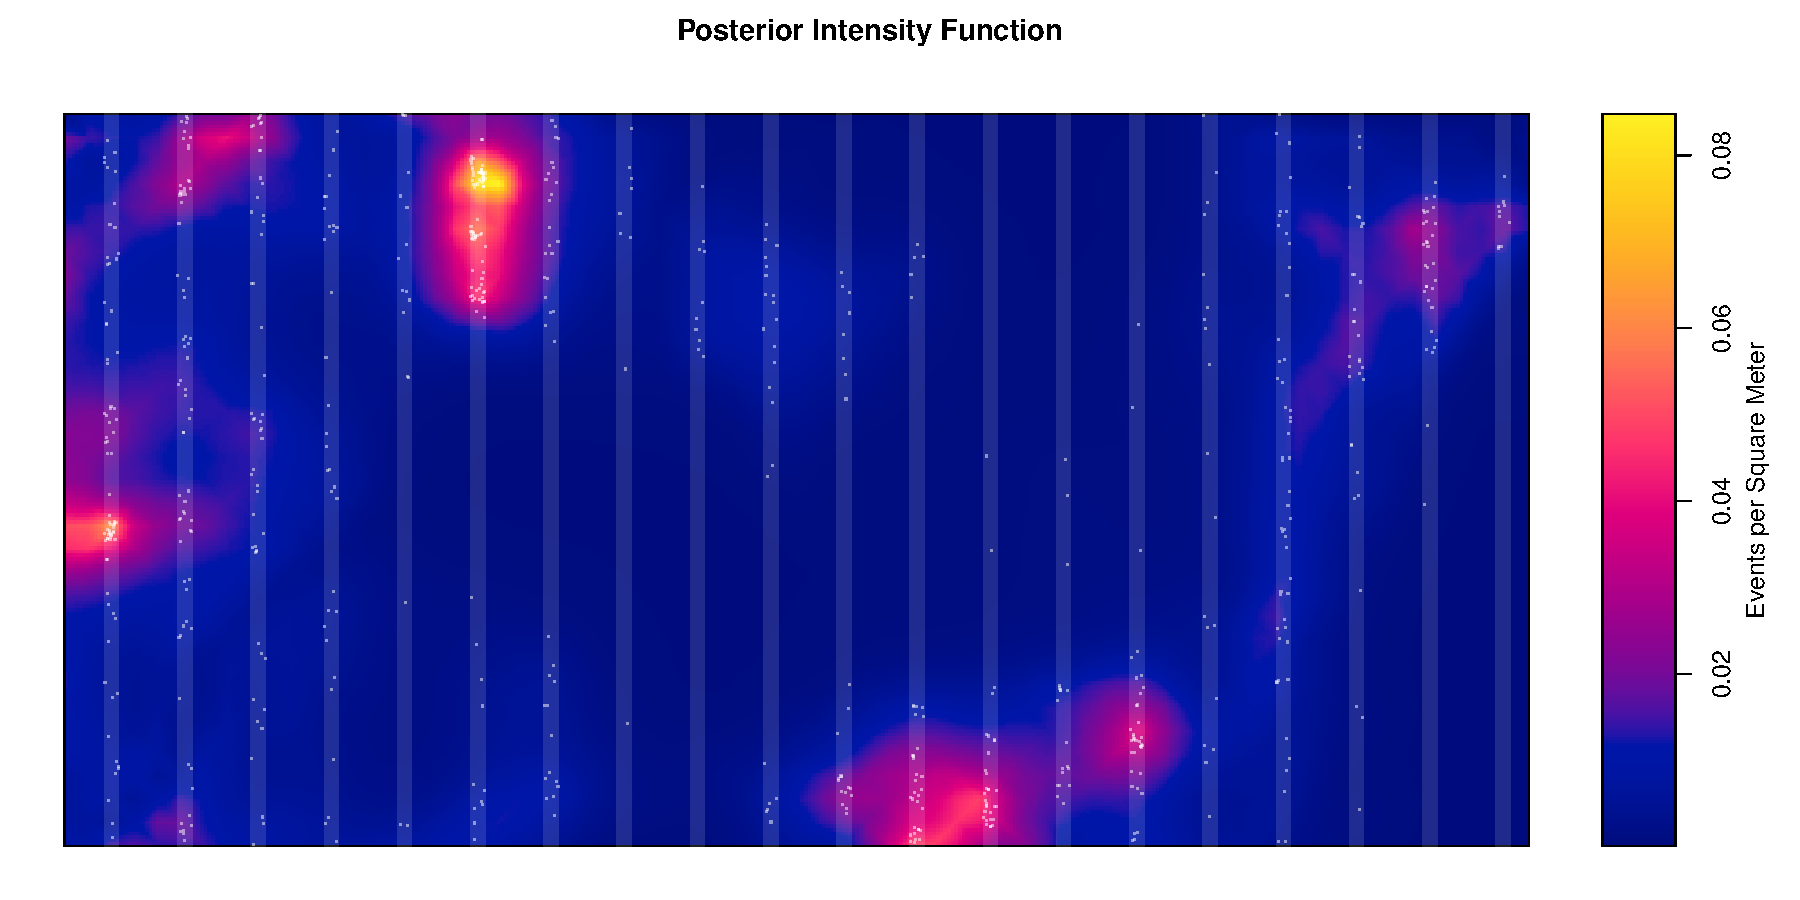
\includegraphics[width=0.9\textwidth]{figures/bei-effort_intensity.pdf}}

\subfloat[Pearson residuals calculated on a grid.]
{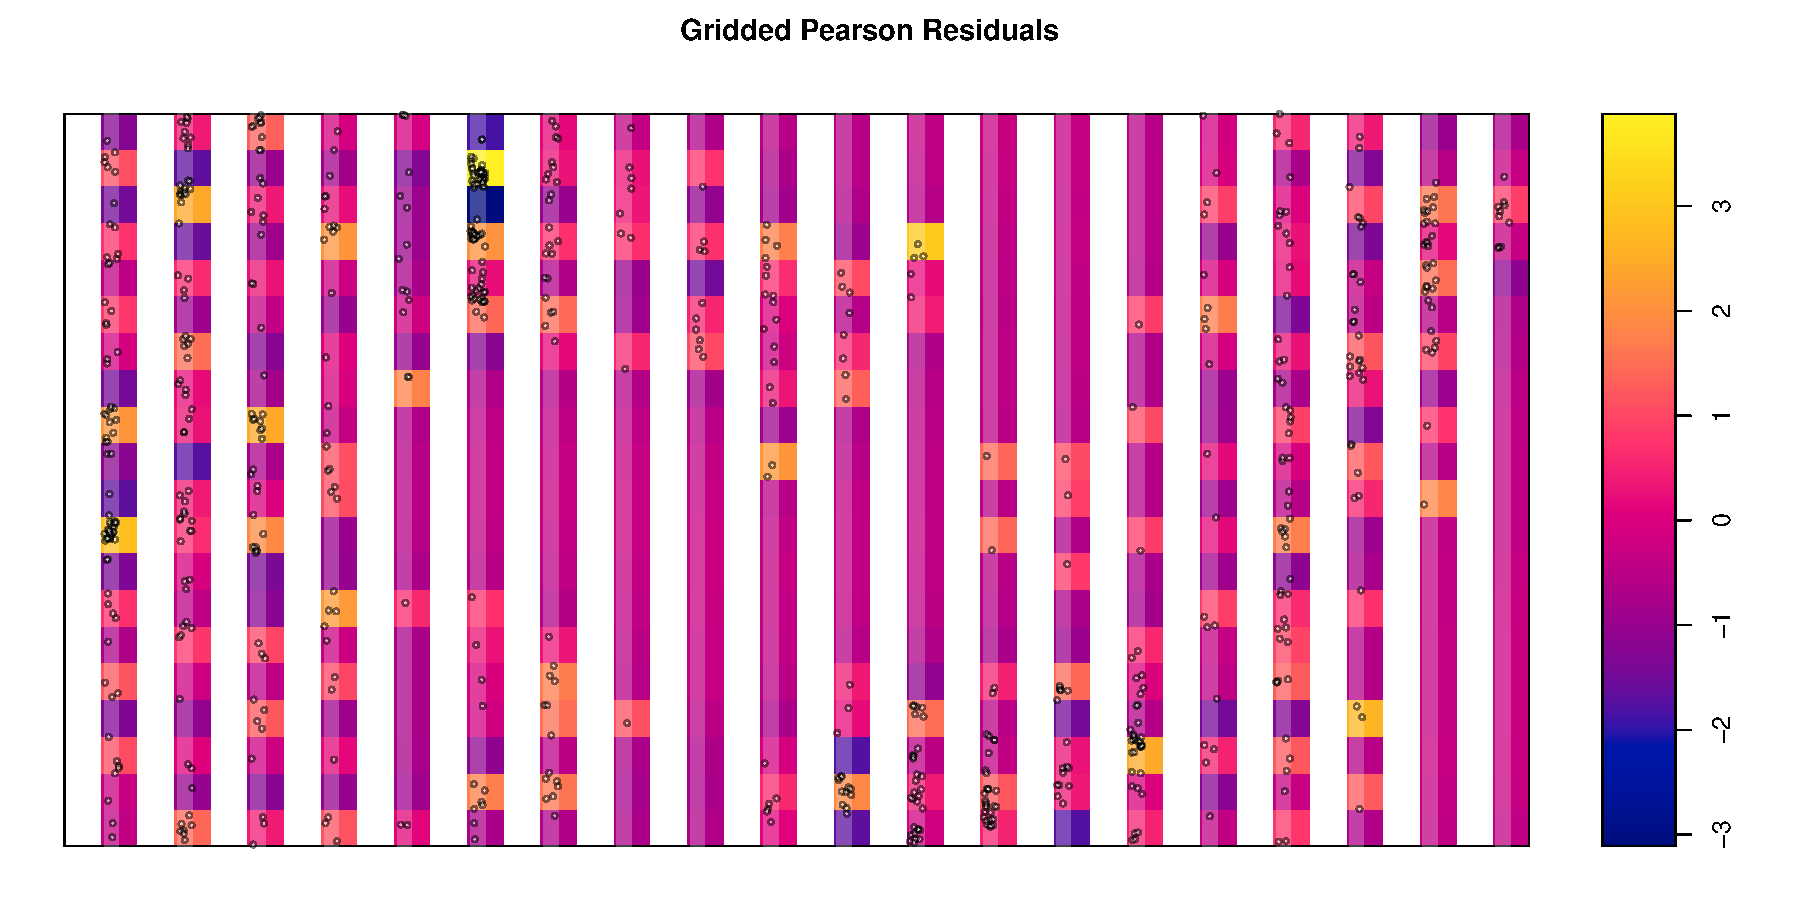
\includegraphics[width=0.9\textwidth]{figures/bei-effort_residuals.pdf}}

\caption{Posterior mean intensity function and Pearson residuals calculated
using the posterior mean intensity from the simulated transect data analysis.}
\label{effortintensity}
\end{figure}


\subsubsection{Model Checking}
\label{effortresid}

To assess the model fit, we computed Pearson residuals on a 40 by 20 lattice of
grid cells. The expected counts were approximated by the multiplying the
posterior mean intensity~(Figure~\ref{effortintensity},~top) at the center of
each grid cell times the observed area within the cell. Cells with no observed
area have undefined residuals and appear white in the
plot~(Figure~\ref{effortintensity},~bottom).

The residuals have low magnitude in the large regions with no observed events
and low posterior intensity. There are more large positive residuals than
large-magnitude negative residuals, including in several places where events
appear to form small clusters. Otherwise, the residuals appear random with no
obvious spatial patterns.


\section{Conclusion and Discussion}
\label{conclusion}

The SPDE approach, Poisson factorization, INLA, and the R-INLA software make
it practical to fit Bayesian spatial LGCP models to real data. It is possible
to make useful maps of spatial predictions with only the pointwise posterior
marginals. The example analyses in this article, using a full real-word dataset and
simulated variable sampling effort applied to the same dataset, show that these
tools can facilitate accurate inference from data collected through sampling.
Both models yielded similar posterior marginal distributions for the
coefficients and the standard deviation. The posterior intervals from the
model fit to the sampled dataset were wider, as expected due to the smaller
area surveyed, but the intervals from both models still have quite a bit of
overlap. For the linear predictor, the posterior mean surfaces from both models
look very similar when mapped across space (Figures \ref{beimean} and
\ref{effortmean}, top panels).

Our example models differ in the posterior distributions of the predicted GP
and the range. The GP prediction surfaces have the same large-scale structure,
but the surface from the model fit to the sampled
data~(Figure~\ref{effortmean}, bottom) is noticeably smoother than the surface
inferred from the complete data~(Figure~\ref{beimean}, bottom).
This is related to the range; the posterior interval for the range when using
the sampled data (161 to 340) is much wider and shifted to the right compared
the interval when using the complete data (137 to 229). The reason for this is
that the LGCP model simply cannot predict detail in regions far from the
observed sections of the site, and there are no data in those unobserved
regions to constrain possible values of the range. Indeed, Simpson et. al.
(2016) discussed this and suggested coarsening the mesh in unsurveyed regions
where extra detail is not needed~\cite{simpsonetal}.

Construction of the mesh requires consideration of both the latent GP and any
covariates. The mesh used in the examples was developed to accurately represent
details in the covariate surfaces, and is finer than needed to describe the
GP. These examples are not particularly complex, but if computation needed
to be further simplified, the mesh could be adaptively coarsened or refined
depending on the local complexity of the covariates.

We have illustrated that, using these tools, spatial mapping based on Bayesian
LGCP models is now practical with useful accuracy in a short amount of time. This
includes when the point pattern is incompletely observed. We look forward to
wider application of spatial LGCP models and future advancements in sampling
for spatial point process models.


%\section*{Acknowledgement(s)}

%An unnumbered section, e.g.\ \verb"\section*{Acknowledgements}", may be used for thanks, etc.\ if required and included \emph{in the non-anonymous version} before any Notes or References.

%\section*{Disclosure statement}

%An unnumbered section, e.g.\ \verb"\section*{Disclosure statement}", may be used to declare any potential conflict of interest and included \emph{in the non-anonymous version} before any Notes or References, after any Acknowledgements and before any Funding information.

%\section*{Funding}

%An unnumbered section, e.g.\ \verb"\section*{Funding}", may be used for grant details, etc.\ if required and included \emph{in the non-anonymous version} before any Notes or References.

%\section*{Notes on contributor(s)}

%An unnumbered section, e.g.\ \verb"\section*{Notes on contributors}", may be included \emph{in the non-anonymous version} if required. A photograph may be added if requested.

%\section*{Nomenclature/Notation}

%An unnumbered section, e.g.\ \verb"\section*{Nomenclature}" (or \verb"\section*{Notation}"), may be included if required, before any Notes or References.

%\section*{Notes}

%An unnumbered `Notes' section may be included before the References (if using the \verb"endnotes" package, use the command \verb"\theendnotes" where the notes are to appear, instead of creating a \verb"\section*").

\bibliographystyle{tfs}
\bibliography{jas-inla-review}

\end{document}
